\documentclass[11pt]{article}
\usepackage{geometry}
\usepackage[onehalfspacing]{setspace}
\usepackage{fancyhdr}
\usepackage{lastpage}
\usepackage{microtype}
\usepackage{hyperref}
\usepackage{xurl}
\usepackage[utf8x]{inputenc}
\usepackage{amsmath}
\usepackage{chngcntr}
\usepackage{graphicx}
\usepackage[colorinlistoftodos]{todonotes}
\usepackage{enumitem}
\usepackage{listings}
\usepackage{filecontents}
\usepackage{verbatim}
\usepackage{eurosym}
\usepackage[export]{adjustbox}
\usepackage[nohyperlinks]{acronym}
\usepackage[pagewise, modulo]{lineno}
\usepackage[format=plain,labelfont={bf,it},textfont=it]{caption}
\usepackage{fancyhdr}
\usepackage[no-math]{fontspec}
\usepackage{amssymb}


% Für keine Abbildungen
%\usepackage{comment}
%\excludecomment{figure}
%\let\endfigure\relax

\hypersetup{
    colorlinks=true,
    linkcolor=black,
    citecolor=blue,
    bookmarksopen=true,
    pdftitle={12g Seminarfacharbeit},
    pdfpagemode=FullScreen,
    }
\geometry{a4paper}

\newcommand{\divides}{\mid}
\newcommand{\notdivides}{\nmid}

\pagestyle{fancy}
\fancyhf{}
\fancypagestyle{plain}{}
\renewcommand{\headrulewidth}{0pt}
\setmainfont{Arial}
\newcommand*\mean[1]{\bar{#1}}

\begin{document}
\begin{titlepage}

    \newcommand{\HRule}{\rule{\linewidth}{0.5mm}}
    \centering
    \textsc{\LARGE Schiller-Gymnasium Hameln}\\[1.5cm]
    \textsc{\Large 12g Seminarfacharbeit}\\[0.5cm]
    \textsc{\Large Mathematik/Physik}\\[0.5cm]
    
    %----------------------------------------------------------------------------------------
    %	TITLE SECTION
    %----------------------------------------------------------------------------------------
    
    \HRule{} \\[0.4cm]
    { \huge \bfseries Umsetzung einer Künstlichen Intelligenz
    \\zur Erkennung handgeschriebener Zahlen}\\[0.4cm]
    \HRule{} \\[1.5cm]
     
    %----------------------------------------------------------------------------------------
    %	AUTHOR SECTION
    %----------------------------------------------------------------------------------------
    
    \begin{minipage}{0.4\textwidth}
    \begin{flushleft} \large
    \emph{Autor:}\\
    Bui Anh Minh Leon Phan\\
    \end{flushleft}
    \end{minipage}
    \begin{minipage}{0.4\textwidth}
    \begin{flushright} \large
    \emph{Tutoren:} \\
    Hr. Fistler, Hr. Dr.\ Kajari\\
    \end{flushright}
    \end{minipage}\\[2cm]
    
    %----------------------------------------------------------------------------------------
    %	DATE SECTION
    %----------------------------------------------------------------------------------------
    
    {\large 27. Januar 2023}\\[2cm]
    
    %----------------------------------------------------------------------------------------
    %	LOGO SECTION
    %----------------------------------------------------------------------------------------
    
    
\includegraphics[width=120pt, keepaspectratio]{images/sghm}\\[2cm]
     
    %----------------------------------------------------------------------------------------
    
    \vfill
    
    \end{titlepage}

\newpage
{
\centering
\Large
\textbf{Schiller-Gymnasium Hameln Europaschule}
}\\[1.5cm]
SF-Kursgruppe: 12g, SFg\\[0.5cm]
Name des Schülers: Bui Anh Minh Leon Phan\\[0.5cm]
Thema: Umsetzung einer Künstlichen Intelligenz zur Erkennung handgeschriebener Zahlen\\[0.5cm]
Namen der Fachlehrkräfte: Herr Dr.\ Kajari, Herr Fistler\\[0.5cm]
Ausgabetermin des Themas: Freitag, der 27.01.2023\\[0.5cm]
Abgabetermin der Facharbeit: Freitag, der 10.03.2023\\[2cm]
Bewertung der Tutoren:
\noindent
\begin{tabular}{ll}
    \makebox[2in]{\hrulefill}
\end{tabular}\\[2cm]
Unterschrift des Schülers:\noindent
\begin{tabular}{ll}
    \makebox[2in]{\hrulefill}
\end{tabular}\\[2cm]
Unterschrift der Fachlehrkraft:\noindent
\begin{tabular}{ll}
    \makebox[2in]{\hrulefill}
\end{tabular}

\newpage

\newgeometry{
    left=50mm,
    right=10mm,
    top=15mm,
    bottom=30mm,
    footskip=15mm
}
\numberwithin{equation}{section}

\renewcommand{\contentsname}{Inhaltsverzeichnis}
\renewcommand{\figurename}{Abbildung}
\tableofcontents
\newpage

\renewcommand{\listfigurename}{Abbildungsverzeichnis}
\listoffigures

\newpage
\section*{Abkürzungs- \& Akronymverzeichnis}

\begin{acronym}
    \acro{2D Convolution}{2D Faltung}
    \acro{Accuracy}{Genauigkeit}
    \acro{Backpropagation}{Fehlerzurückführung}
    \acro{CNN}{Faltendes Neuronales Netzwerk}
    \acro{Cross Correlation}{Kreuzkorrelation}
    \acro{Cross Entropy}{Kreuzentropie}
    \acro{KI}{Künstliche Intelligenz}
    \acro{FNN}{Vorwärtsgerichtetes Neuronales Netzwerk}
    \acro{Overfitting}{Überanpassung}
    \acro{ReLU}{Rectified Linear Unit}
    \acro{SGD}{Stochastisches Gradientenverfahren}
    \acro{Underfitting}{Unteranpassung}
    
\end{acronym}
\newpage

\renewcommand\linenumberfont{\normalfont\small}
\setlength\linenumbersep{1cm}
\linenumbers{}
\setcounter{page}{1}
\rfoot{Seite {\thepage}}

\section{Einleitung}
Das menschliche Gehirn wird von vielen nicht richtig verstanden. Wird Abbildung 1 betrachtet, dann erkennt der Beobachter die Zahl 74290,
was leicht zu bestimmen ist. Wenn aber der Vorgang versucht wird zu erklären, so wird es klar, dass es nicht ganz einfach ist
und dass es komplex werden kann.
\begin{figure}[h]
    \centering
    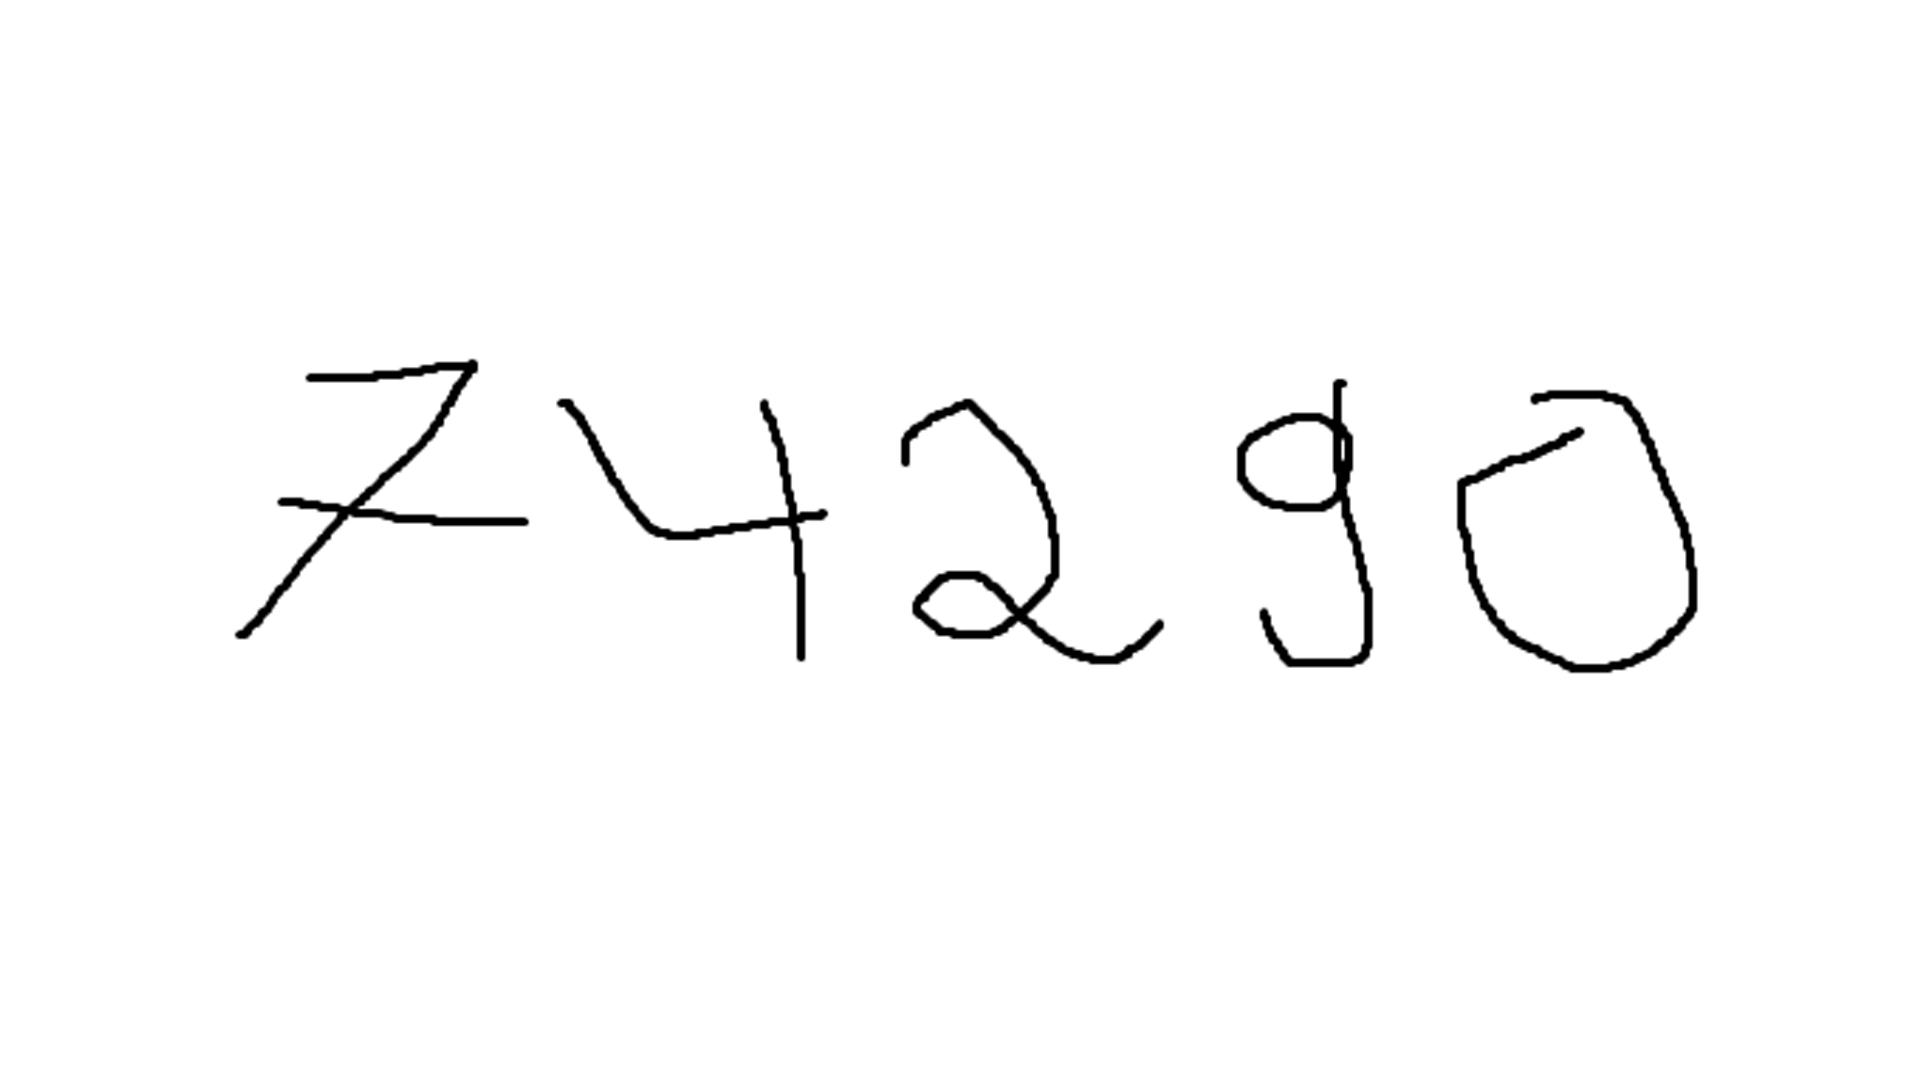
\includegraphics[width=230pt, keepaspectratio]{images/zahlen}
    \caption[Handgeschriebene]{Erkennbar ist die handgeschriebene Zahl 74290.}
\end{figure}
Die Problemstellung lautet: Wie können handgeschriebene Zahlen erkannt werden.
Dieses Thema ist von besonderem Interesse, weil das Verständnis zur Funktionsweise eines menschlichen Gehirns zum Teil vertieft werden kann.
Außerdem wird der Mechanismus eines Textscanners verstanden, was im Alltag von den Meisten unbewusst benutzt wird.
Viele Forscher versuchten deshalb in der Vergangenheit nach Problemlösungen zu suchen. Ein Ansatz wäre das Herausfinden
der Struktur der einzelnen Zahlen und damit die Unterscheidungen zwischen den Zahlen.
Doch jedes Merkmal einer Zahl selber herauszufinden und dann speziell für jede Zahl das zu programmieren, kann
anstrengend sein und lange dauern. Mithilfe einer Künstlichen Intelligenz (KI) kann die Erkennung von handgeschriebenen Zahlen ermöglicht werden. 
Schon heute werden KI-Systeme in unseren Alltag integriert, wie zum Beispiel Textübersetzer oder Gesichtserkennung im Smartphone. Da die KI solche
komplexe Strukturen erkennen kann, welche ein Mensch vielleicht nicht erkennt, wird in der Facharbeit für die Erkennung der handgeschriebenen Zahlen eine KI programmiert.
So weckte das Thema mein Interesse, mich damit zu beschäftigen, da nur anhand der Mathematik die Entscheidungsprozesse dargestellt werden könnnen.
Auch ist die Facharbeit von Vorteil für mich, da ich an dem Bundeswettbewerb-KI teilnehmen möchte~\cite{10}.
Ziel der Facharbeit ist es, eine KI zu programmieren, die handgeschriebene Zahlen mit einer Wahrscheinlichkeit von mindestens 97\% bestimmen kann.
Um dies umsetzen zu können, wird zunächst der Begriff KI definiert und sich mit den verschiedenen Arten von KIen,
welche Funktion jede einzelne Art besitzt, auseinandergesetzt. Die angewendete Lernmethode wird genauer erläutert.
Danach wird in Kapitel 3 mehrschichtiges Lernen erklärt. Zudem werden Voraussetzungen für diese Methodik genannt. Im Anschluss wird in Kapitel 4
der Aufbau eines faltenden Neuronalen Netzwerkes dargestellt und die Funktionsweise mathematisch näher gebracht. Dabei wird darauf eingegangen, wie eine KI
lernt und wie sie bestimmte Merkmale der Zahlen erkennen kann mithilfe von 2D Faltung (2D Convolution). Der Begriff Merkmal wird auch in dem Kapitel erläutert.
Mithilfe der Theorie wird dann in Kapitel 5 die KI umgesetzt und programmiert. Dabei wird sie ausgewertet für analysiert, worauf bei der Lernphase
geachtet werden muss. Dies kann durch die Analyse optimiert werden. Zum Schluss wird angeschaut, ob das Ziel der Facharbeit erreicht wurde und welche
Verbesserungsvorschlägen eingefügt werden können, damit die KI eine höhere Wahrscheinlichkeit hat, die Zahl richtig vorherzusagen.


\section{Künstliche Intelligenz}
Der Begriff Künstliche Intelligenz (KI) ist sehr schwer definierbar, denn es mangelt an der Definition der Bezeichnung Intelligenz.
Allgemein kann KI definiert werden als der Versuch, bestimmte Entscheidungsstrukturen von Menschen mithilfe von
Algorithmen nachzubilden~\cite{4}. Manche Experten behaupten aber auch, dass eine KI nicht gleich einer KI ist, sondern sie in zwei Bereiche unterteilt werden kann.
Dabei wird die KI zwischen einer starken KI und einer schwachen KI unterschieden. Schwache KIen sind nur in bestimmten Teilbereichen in der Lage,
an die menschliche Intelligenz heranzukommen. Doch sie sind nicht anpassungsfähig. Das bedeutet, dass eine schwache KI, die zum Beispiel auf Schach
spezialisiert wurde, nur die Intelligenz im Bereich Schach besitzt. Selbstständiges Fahren ist mit dieser KI nicht möglich. Dafür muss eine
andere KI spezialisiert werden, damit sie selbstständig fahren kann. Dagegen kann eine starke KI sich an derzeitige Situationen anpassen~\cite{2}.
Solche starken KIen sind heutzutage noch nicht umsetzbar und es wird ausschließlich daran geforscht.
Die schwache KI, die in der Facharbeit speziell zur Erkennung von handgeschriebenen Zahlen programmiert wird, kann in 2 Teilbereichen
unterteilt werden.
\begin{figure}[h]
    \centering
    \includegraphics[width=250pt, keepaspectratio]{images/ki\_kategorie}
    \caption[Unterkategorien der Künstliche Intelligenz~\cite{4}]{Die KI besitzt 2 Unterkategorien: Maschinelles Lernen und mehrschichtiges Lernen~\cite{4}.}
\end{figure}
Eine Unterkategorie der KI wäre der Bereich maschinelles Lernen. Maschinelles Lernen versucht mithilfe von Algorithmen mit einer großen Anzahl von
Daten Muster zu erkennen. Dazu werden die aus den Daten gewonnene Erkenntnisse zur Problemlösung verwendet oder der Algorithmus wird auf
die Daten zugeschnitten und verallgemeinert.
Der zweite Teilbereich wäre mehrschichtiges Lernen, das dem maschinellen Lernen sehr ähnelt. Der Unterschied liegt aber an der Art und Weise, wie
sie mit den Daten arbeitet. Mehrschichtiges Lernen versucht das menschliche Gehirn durch ein Künstliches Neuronales Netzwerk zu imitieren.
Durch das Imitieren sind die Strukturen vom mehrschichtigen Lernen merklich komplexer als die vom maschinellen Lernen, denn
maschinelles Lernen basiert nur auf Algorithmen, die leichter verständlicher sind als das menschliche Gehirn. Deswegen sind
sehr große Datensätze von Vorteil für mehrschichtiges Lernen, da deutlich mehr Merkmale der Daten erkannt werden. So basiert die KI auf
mehrschichtigem Lernen in der Facharbeit.
\subsection{Überwachtes Lernen}
Überwachtes Lernen ist eine Methode, wie die KI mit Daten lernen kann. Dazu hat die Datei 2 wichtige Merkmale, nämlich die Eingabe und die
Ausgabe. Die KI führt mit den Eingaben eine Lernstrategie aus, in dem Fall einen Algorithmus, woraus am Ende eine Ausgabe resultiert. Mit der Ausgabe der Datei wird nun überprüft, ob
die Antwort, die die KI ausgegeben hat, übereinstimmt.
\begin{figure}[h]
    \centering
    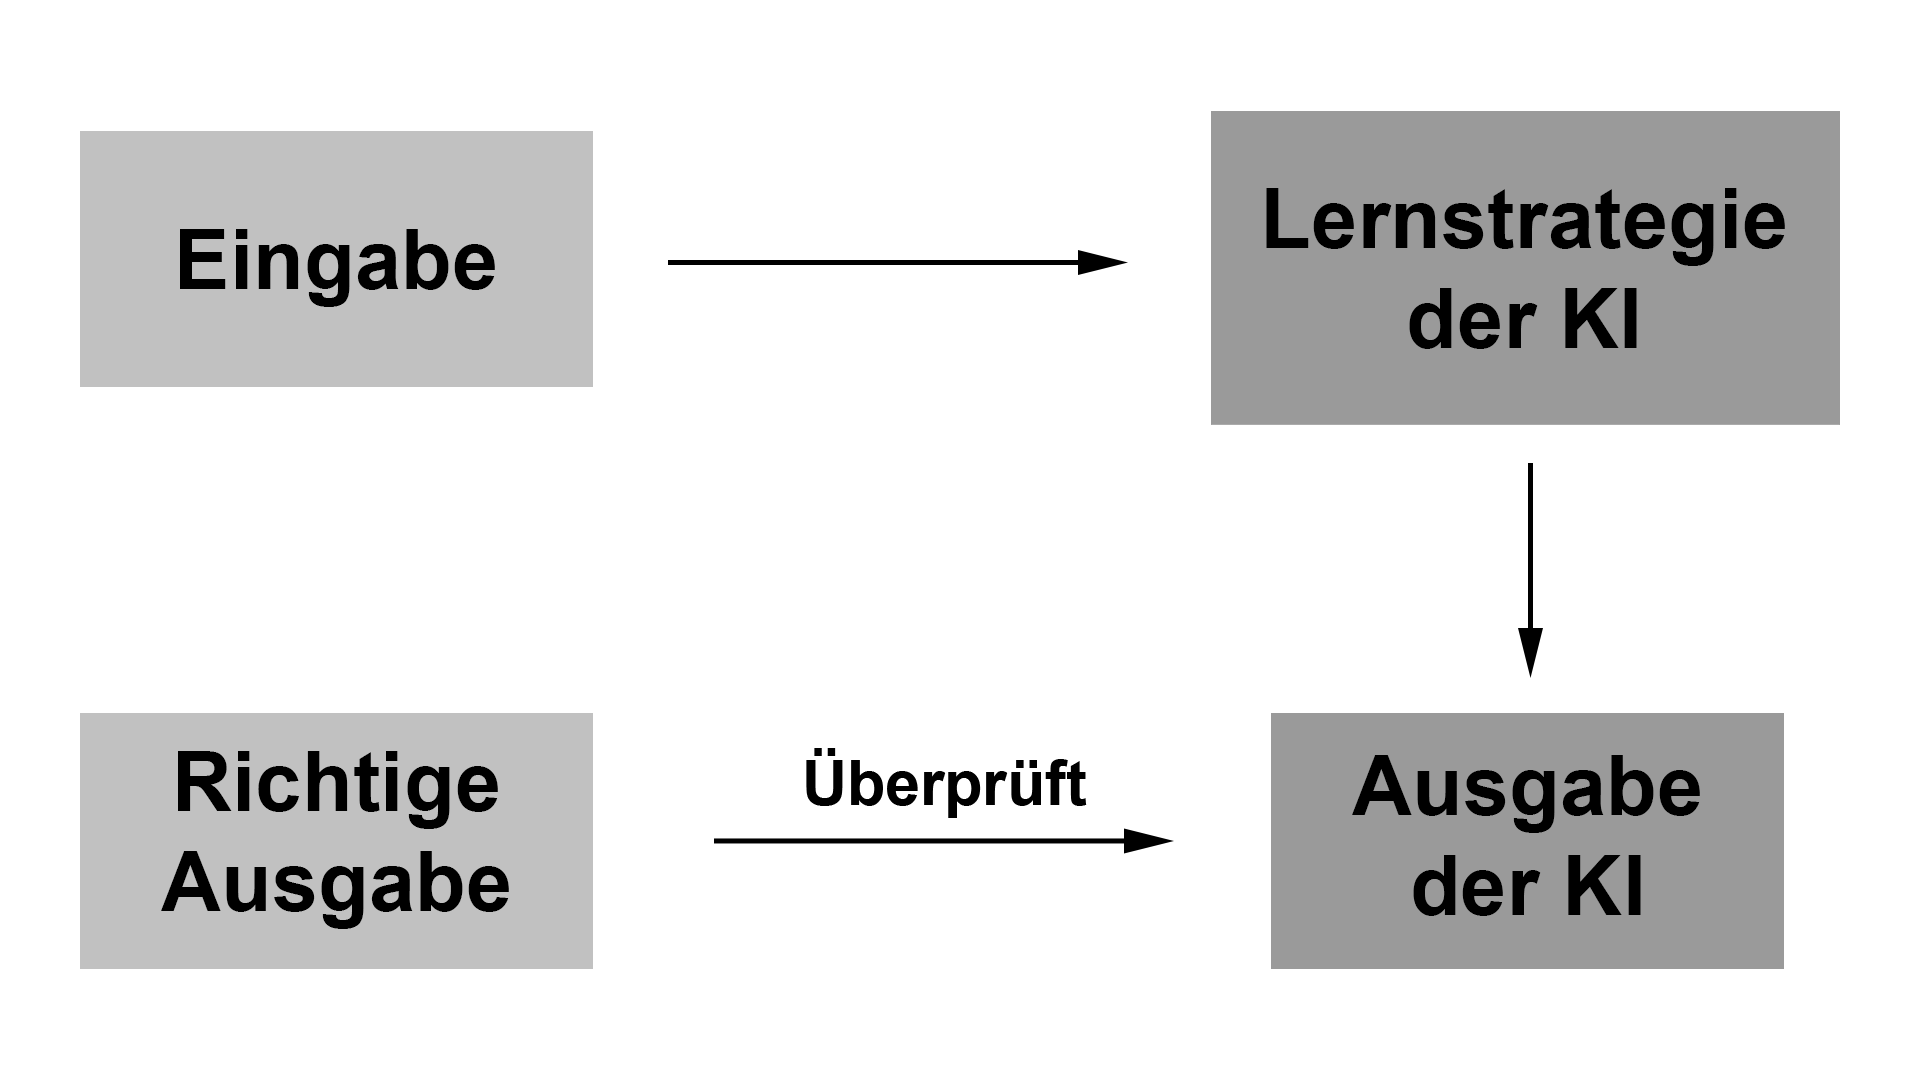
\includegraphics[width=300pt, keepaspectratio]{images/slearning}
    \caption[Ablauf eines überwachtes Lernen~\cite{7}]{Zuerst wird die Eingabe verwendet, um zu lernen. Dafür verwendet die KI eine Lernstrategie. Nachdem etwas
    ausgegeben wurden, werden die Ausgaben verglichen~\cite{7}.}
\end{figure}
Falls sie nicht übereinstimmt, lernt die KI aus den Fehlern und verbessert sich
dadurch~\cite{7}. Überwachtes Lernen ist eine angemessene Methode für das Problem der Facharbeit, da die Antwort, die die KI ausgibt, sich mit der richtigen Antwort decken muss.
Dadurch wird die Fehlerquote der KI möglichst kleingehalten, sodass eine genaue Erkennung der handgeschrieben Zahlen gelingen kann.
Dabei ist anzumerken, dass die KI zwei Arten von Lösungen angeben kann.
Jeder Zahl wird eine eigene Klasse zugeordnet. In dem Fall gäbe es 9 Klassen für jede Ziffer von 0-9.
Die KI gibt aus, um welche Klasse es sich handelt.
In dem Fall wird die sogenannte Klassifikation als Lösungsart akzeptiert.

\section{Voraussetzung für mehrschichtiges Lernen}
Im Gegensatz zum maschinellem Lernen braucht das mehrschichtige Lernen sehr viele Daten: Es wird von mindestens 10000 Daten gesprochen.
Im Vergleich zum maschinellen Lernen schneidet mehrschichtiges Lernen bei größeren Datensätzen besser ab. Wiederum verbraucht diese Methode mehr
Rechenleistung. So kann es mehrere Tage oder Wochen dauern, bis die KI fertig gelernt hat und einsatzbereit ist. Auch braucht die KI ein Modell zum
Lernen, ein Künstliches Neuronales Netzwerk. Dafür gibt es verschieden Modelle von Netzwerken. Die Auswahl des Modells für die KI wird später im Kapitel
~\ref{nn} erläutert.

\subsection{Datensatz}
Datensätze sind für KIen das wichtigste Werkzeug zum Lernen. Denn die Qualität des Datensatzes bestimmt die Lerneffizienz der KI.\@
Je schlechter die Qualität ist, desto schlechter lernt auch die KI.\@ Ein wichtiges Merkmal für die Qualität sind die Auflösung, die Anzahl der Daten und die Variabilität.
Für mehrschichtiges Lernen wird ein großer Datensatz gebraucht. Dabei wird für die Problemlösung der Datensatz von Yann LeCun gewählt, dass sich MNIST Database nennt~\cite{3}.
Dieser besitzt insgesamt 70000 Bilder mit handgeschrieben Zahlen, die die Werte zwischen 0 und 9 besitzen. Jedes Bild hat ein 28$\times$28 Pixel
Format und ist farblos. Die Bilder werden nur mit der Hellgikeit zwischen 0 und 255 dargestellt. Außerdem hat jedes Bild einen Wert, um welche Zahl
es sich handelt, damit später geprüft werden kann, ob die KI die Zahl richtig erkannt hat oder ob sie falsch liegt.
\begin{figure}[h]
    \centering
    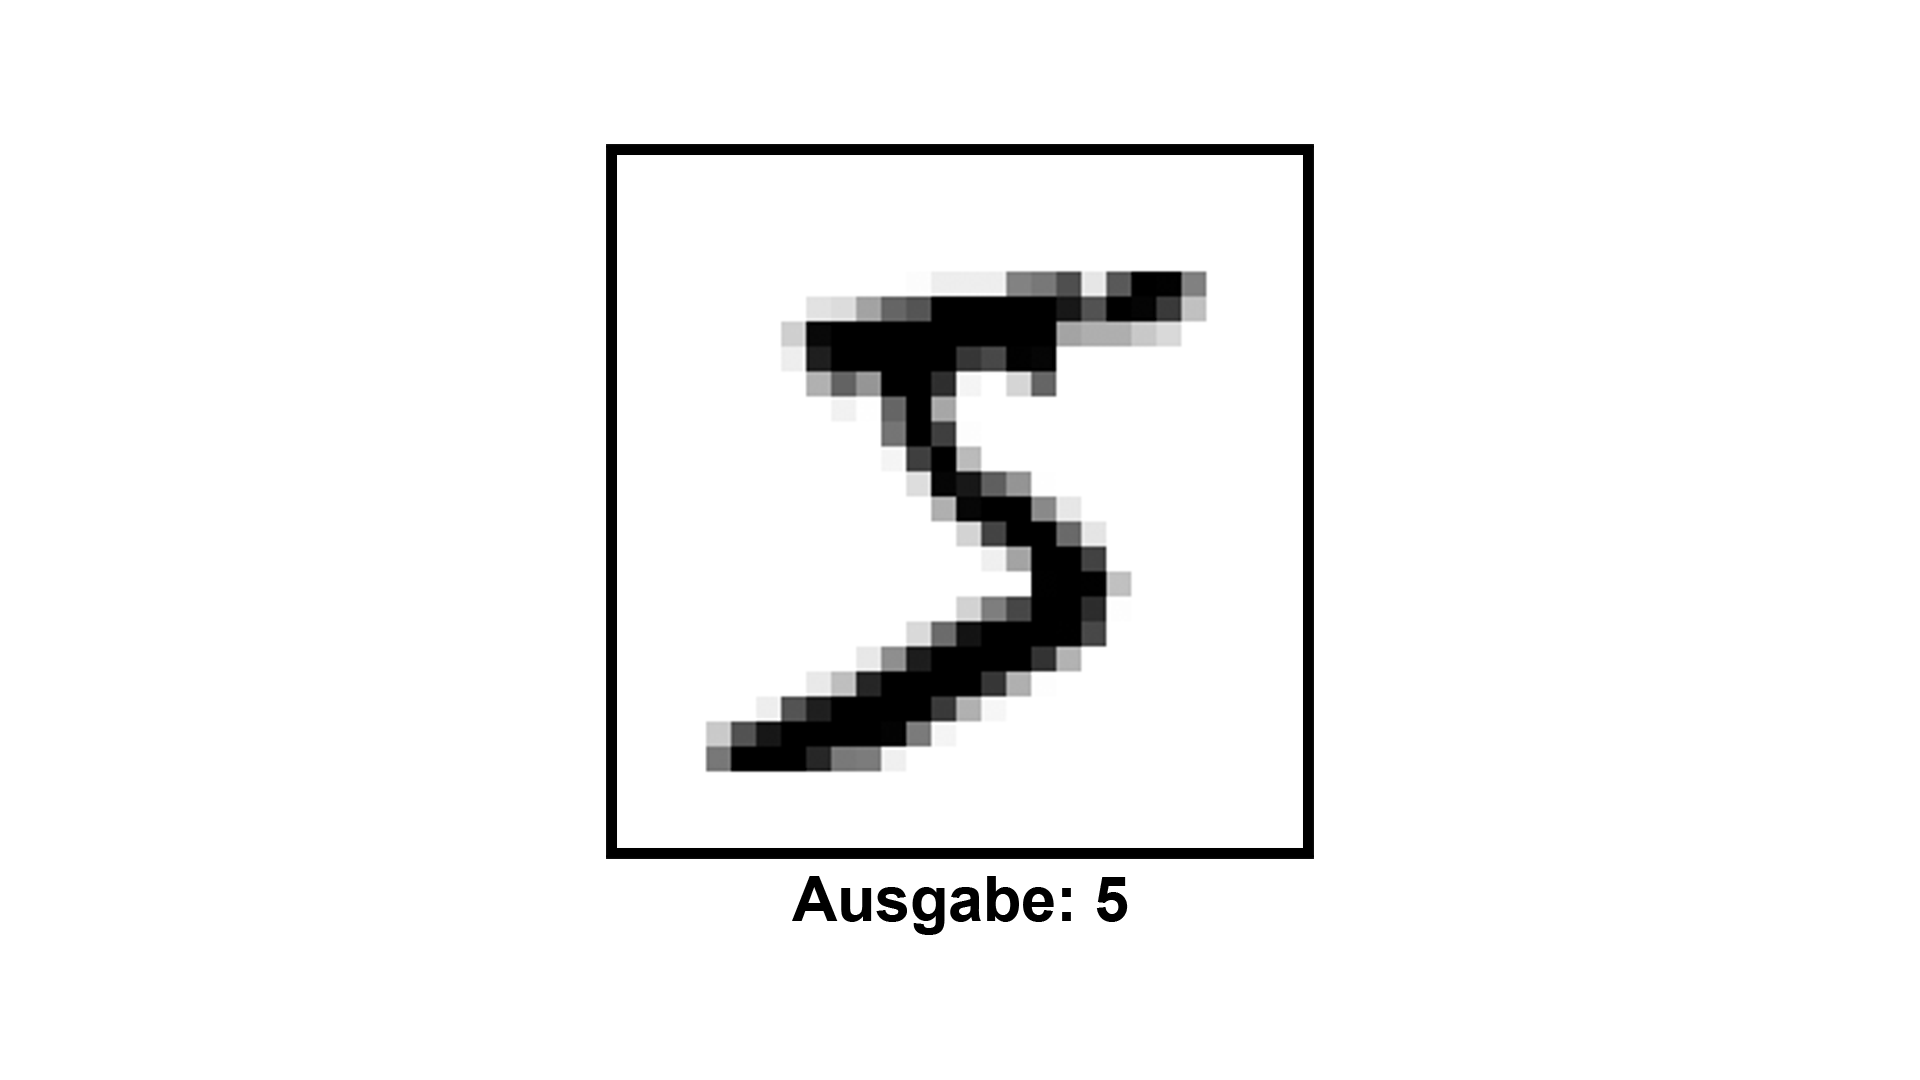
\includegraphics[width=250pt, keepaspectratio]{images/number}
    \caption[Handgeschriebene Zahl 5~\cite{3}]{Handgeschriebene Zahl als Abbildung in 28\times28 Pixeln dargestellt, dabei ist die richtige Ausgabe die Zahl 5~\cite{3}.}
\end{figure}
Nach den vorhergenannten Kriterien ist der Datensatz gut zum Lernen, denn die Auflösung des Bildes ist ausreichend und die Variabilität ist vielfältig.
Außerdem sind 70000 Bilder ausreichend für diese Problemstellung.

\subsection{Künstliches Neuronales Netzwerk}\label{nn}
Im menschlichen Gehirn befinden sich großen Mengen von Neuronen, die miteinander interagieren. 
Das Neuron besteht aus drei relevanten Komponenten. Die erste Komponente besteht aus Empfängern, die Signale von anderen verbundenen Neuronen empfängt.
Sie werden auch Dendriten genannt. Eine weitere Komponente wären die Synapsen. Die Aufgabe ist es, sogenannte Neurotransmitter an anderen verbundenen Neuronen
weiterzuleiten, falls das Signal ankommen sollte. Damit das Signal ankommt, braucht es die dritte Komponente und zwar das Axon. Das Axon wird als Leitungsbahn
verwendet, um Signale transportieren zu können und besteht aus einer langen dünnen Röhre. Diese Röhre kann das Signal zu den Synapsen weiterleiten, unter Voraussetzung, dass der Schwellenwert erreicht ist.
Falls er nicht erreicht werden sollte, wird das Signal abgebrochen. Der Schwellenwert wird erreicht, wenn genug Neurotransmitter vorhanden sind.
Sobald das Signal ankommt, werden die Neurotransmitter
ausgeschüttet und die Dendriten der anderen verbundenen Neuronen nehmen sie auf.
Dadurch ändert sich die Struktur des Neurons und es kommt wieder zur Entscheidung, ob das Signal weitergeleitet werden soll oder abgebrochen wird.
Es entsteht eine Kettenreaktion~\cite{11}.
\begin{figure}[h]
    \centering
    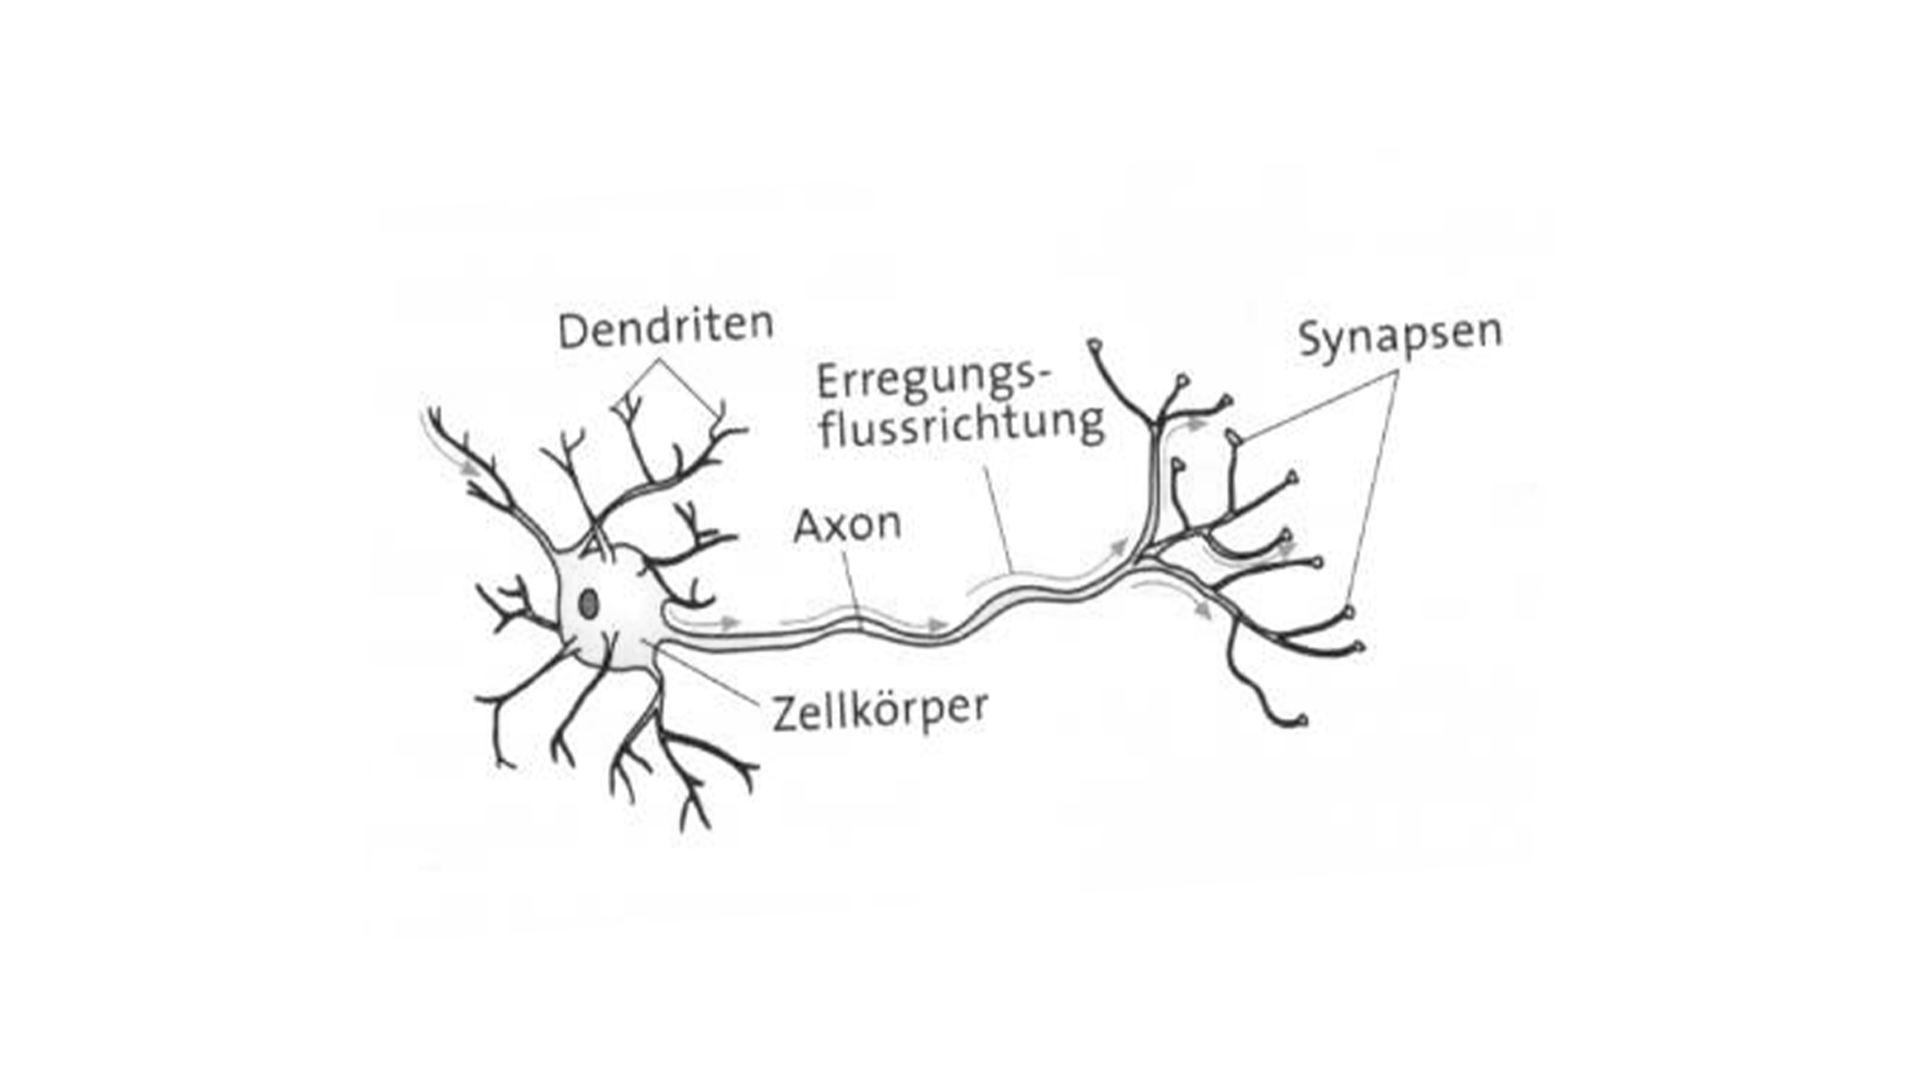
\includegraphics[width=300pt, keepaspectratio]{images/neuron}
    \caption[Aufbau eines Neuron~\cite{11}]{Das einzelne Neuron sendet mithilfe der Synapsen Signale an die verbundenen Neuronen, die diese Signale mit den Dendriten aufnehmen~\cite{11}.}
\end{figure}
Da das menschliche Gehirn imitiert werden soll, werden künstliche Neuronen erschaffen, die einen Wert von den vorherigen künstlichen Neuronen verarbeiten.
Durch die ganzen Verbindungen zwischen den Neuronen wird das auch als Netzwerk bezeichnet. Viele Eigenschaften der Neuronen werden mitgenommen, wie zum Beispiel die Dendriten, die Synapsen sowie
der Schwellenwert in der Informatik auch Bias genannt. Der Bias spielt im Kapitel~\ref{fcnn} eine Rolle. Unterschied ist aber,
dass die künstlichen Neuronen ihre Struktur nicht ändern können, dafür können ihnen Werte gegeben werden. Das bedeutet, dass das künstliche Neuron
negative Werte annehmen kann, was bei den Neuronen nicht der Fall ist, da das Axon nur das Signal weiterleiten oder abbrechen kann. Sie können auch mit 0 und 1 bezeichnet werden~\cite{5}.
\begin{figure}[h]
    \centering
    \includegraphics[width=250pt, keepaspectratio]{images/neural\_network}
    \caption[Künstliches Neuronales Netzwerk]{Künstliches Neuronales Netzwerk mit insgesamt 37 künstliche Neuronen in 6 Schichten verteilt.}\label{fnnpic}
\end{figure}
Das Netzwerk kann unterschiedliche Anordnungen von künstlichen Neuronen besitzen. Die geeignetste Anordnung nennt sich
Faltendes Neuronales Netzwerk (CNN), denn sie wird häufig für Bildererkennung verwendet. Grund dafür ist die Extrahierung der Merkmale
des Bildes. Denn bevor das Bild an die künstlichen Neuronen weitergeleitet werden, werden unnötige Merkmale mithilfe von Konvolution aus dem Bild entfernt, sodass der
Lernprozess der KI auf das Wichtigste begrenzt wird~\cite{12}. Welche Merkmale eines Bildes gemeint sind, wird im Kapitel~\ref{feature} verdeutlicht.

\section{Faltendes Neuronales Netzwerk}

Das CNN kann in zwei Bereichen gegliedert werden. Im ersten Bereich werden Merkmale des Bildes extrahiert, wie zum Beispiel Ecken, Kurven, usw. Diese nennt sich Feature Extraction.
Die Extrahierung wird durch 2D Convolution berechnet. Im zweiten Bereich werden die
wichtigen Merkmale aus der Feature Extraction in die sogenannte Klassifikationsebene weitergeleitet. Dort fängt der Lernprozess
der KI an, die dann am Ende des Netzwerkes eine Klasse ausgibt~\cite{12}.

\subsection{Klassifikationsebene}\label{fcnn}
In der Klassifikationsebene befindet sich das Künstliche Neuronale Netzwerk, das eine ähnliche Struktur wie bei Abbildung~\ref{fnnpic} hat.
Diese Struktur nennt sich auch Vorwärtsgerichtetes Neuronales Netzwerk (FNN) und ist in mehreren Schichten aufgebaut~\cite{5}. In Abbildung~\ref{fnnpic} wäre die Anzahl
der Schichten $A = 6$. Die erste Schicht nennt sich Eingabeschicht, denn von dort kommen die Daten in die Neuronen rein, während bei
der n Schicht die KI ein Ergebnis ausgibt. Diese Schicht heißt Ausgabeschicht. Die Schichten dazwischen werden ausgeblendete Schichten genannt.
Die ausgeblendete Schichten sind wichtige Teile des Netzwerkes, denn durch diese werden Merkmale gesucht und analysiert.
Das gibt nochmal eine deutlich stärkere Lerntiefe für die KI, da mehr Schnittstellen zwischen den künstlichen Neuronen existieren.
Das Netzwerk läuft also von links nach rechts durch.\@ Die einzelne Neuronen können einen Wert besitzen. Dies wird als $ x_{i}^{(\alpha,\beta)} $ definiert,
wobei $ \alpha \in \{1,\ldots,A\} $ gilt. Der Index $i$ beschreibt um welches Neuron in der Schicht $\alpha$ es sich dabei handelt. Der Wert $\beta$ wird später
verwendet. Für die Einheitlichkeit der Formeln steht in dem Fall $\beta$ in der Variable. In der Klassifikationsebene bleibt $\beta = 1$. Dieser Wert
lässt sich aus den ganzen Verbindungen der vorherigen Schicht berechnen, indem sie wie in Abbildung~\ref{connection} addiert werden. Dabei werden
die einzelne Werte $ x_{j}^{(\alpha-1,1)} $ mit einem Gewicht $ w_{i,j}^{(\alpha,1)} $ multipliziert, womit $ j \in \{1,\ldots,N_{\alpha-1}\} $ gilt~\cite{5}.
$ N_{\alpha} $ beschreibt die Anzahl der Neuronen auf der Schicht $\alpha$.
\begin{figure}[h]
    \centering
    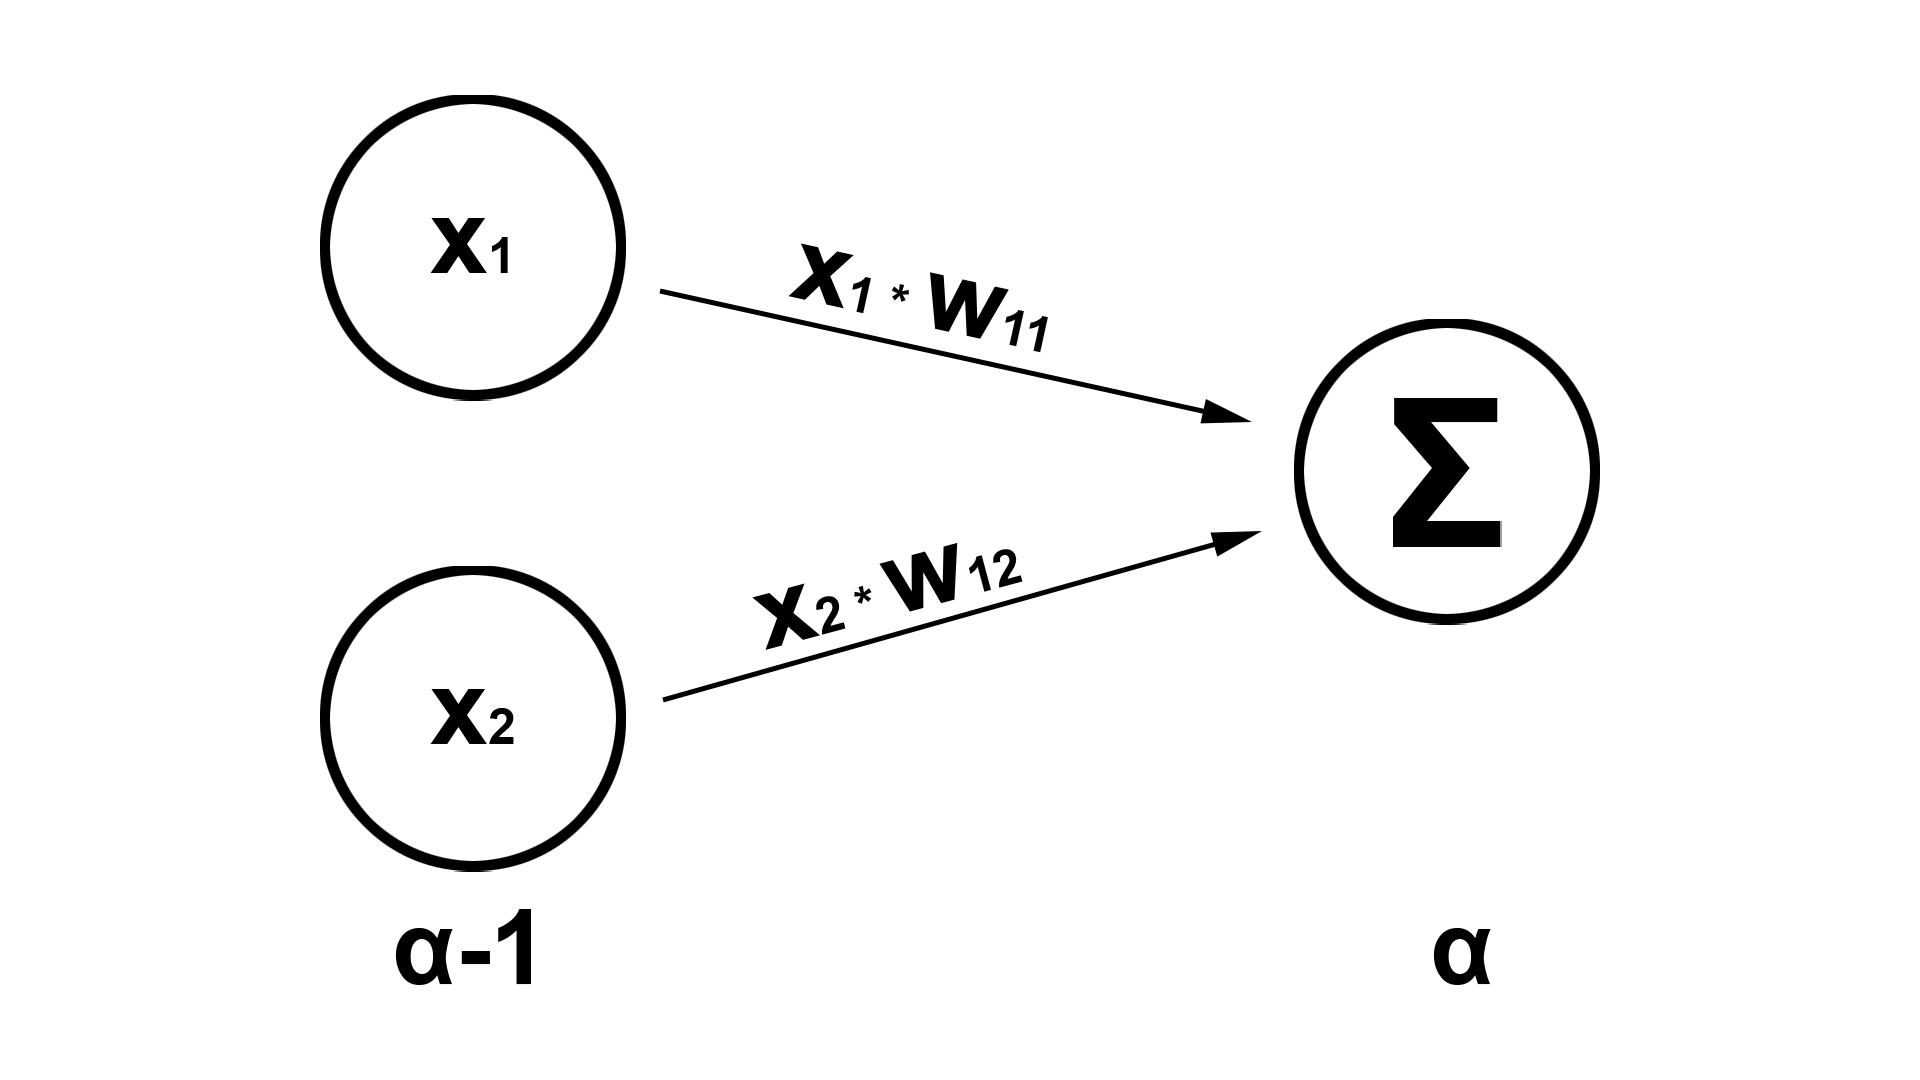
\includegraphics[width=250pt, keepaspectratio]{images/verbindung}
    \caption[Verbindungen zwischen den Neuronen]{Die Verbindungen zwischen den Neuronen werden mit den Parameter $w$ erweitert.}\label{connection}
\end{figure}
Allgemein gilt dann für die Berechnung:
\begin{equation}
    \label{xwithoutfunction}
    \bar{x}_{i}^{(\alpha,1)} := \sum_{j=1}^{N_{\alpha-1}} w_{i,j}^{(\alpha,1)} x_{j}^{(\alpha-1,1)} + b_{i}^{(\alpha,1)} \quad i \in \{1,\ldots,N_{\alpha}\}, j \in \{1,\ldots,N_{\alpha-1}\}.
\end{equation}
Dies ist für die Berechnung eines Neurons $i$ in der Schicht $\alpha$.
Das $ b_{i}^{(\alpha,1)} $ in der Gleichung steht für Bias und ist ein weiterer Parameter zum Einstellen wie das Gewicht. Beide spielen hier eine wichtige Rolle
für das Weiterleiten der Neuronen. Das Gewicht entscheidet, wie wichtig der Wert vom Neuron ist. Je höher der Wert ist, desto entscheidender
ist das Neuron. Wichtig ist anzumerken, dass die Gewichte und die Biases verstellbare Parameter sind, die für das Lernen der KI eine wichtige Rolle
spielen. Damit die KI lernen kann, müssen die Parameter $w$ und $b$ optimal gesetzt werden, sodass die KI richtige Voraussagen treffen kann, um welche Zahl es sich dabei handelt.
Dafür wird die Fehlerzurückführung (Backpropagation) verwendet~\cite{5}. Erstmal werden nur die partiellen Ableitungen berechnet. Warum sie gebraucht werden, wird im Kapitel~\ref{back} genauer
erläutert. So kann in der Gleichung~\ref{xwithoutfunction} partiell nach drei Variablen der Funktion $C(\vec{y},\vec{x}^{(A,1)})$ abgeleitet werden: $x_{j}^{(\alpha-1,1)}$, $w_{i,j}^{(\alpha,1)}$ und $b_{i}^{(\alpha,1)}$.
Auch die Funktion $C(\vec{y},\vec{x}^{(A,1)})$ wird in Kapitel~\ref{lost} genauer erläutert.
Folgendes ergibt sich:
\begin{equation}
    \frac{\partial C}{\partial b_i^{(\alpha,1)}} = \frac{\partial C}{\partial \bar{x}_i^{(\alpha,1)}},
\end{equation}
\begin{equation}
    \frac{\partial C}{\partial w_{i,j}^{(\alpha,1)}} = \frac{\partial C}{\partial \bar{x}_i^{(\alpha,1)}} x_j^{(\alpha-1,1)},
    \label{w}
\end{equation}
\begin{equation}
    \frac{\partial C}{\partial x_{j}^{(\alpha-1,1)}} = \sum_{i=1}^{N_{\alpha}} \frac{\partial C}{\partial \bar{x}_i^{(\alpha,1)}} w_{i,j}^{(\alpha,1)}.
\end{equation}
Eine weitere Sache, die hinzugefügt werden muss, ist die Aktivierungsfunktion, denn sie gibt dem Netzwerk eine Komplexität~\cite{7}.
Ohne diese Komplexität wäre das Netzwerk linear, weswegen die KI nur eine lineare Regression durchführen können.
In Abbildung~\ref{regressionpic} ist die Regression bei einer
nicht lineare Struktur deutlich besser als die einer lineare Struktur.
\begin{figure}[h]
    \centering
    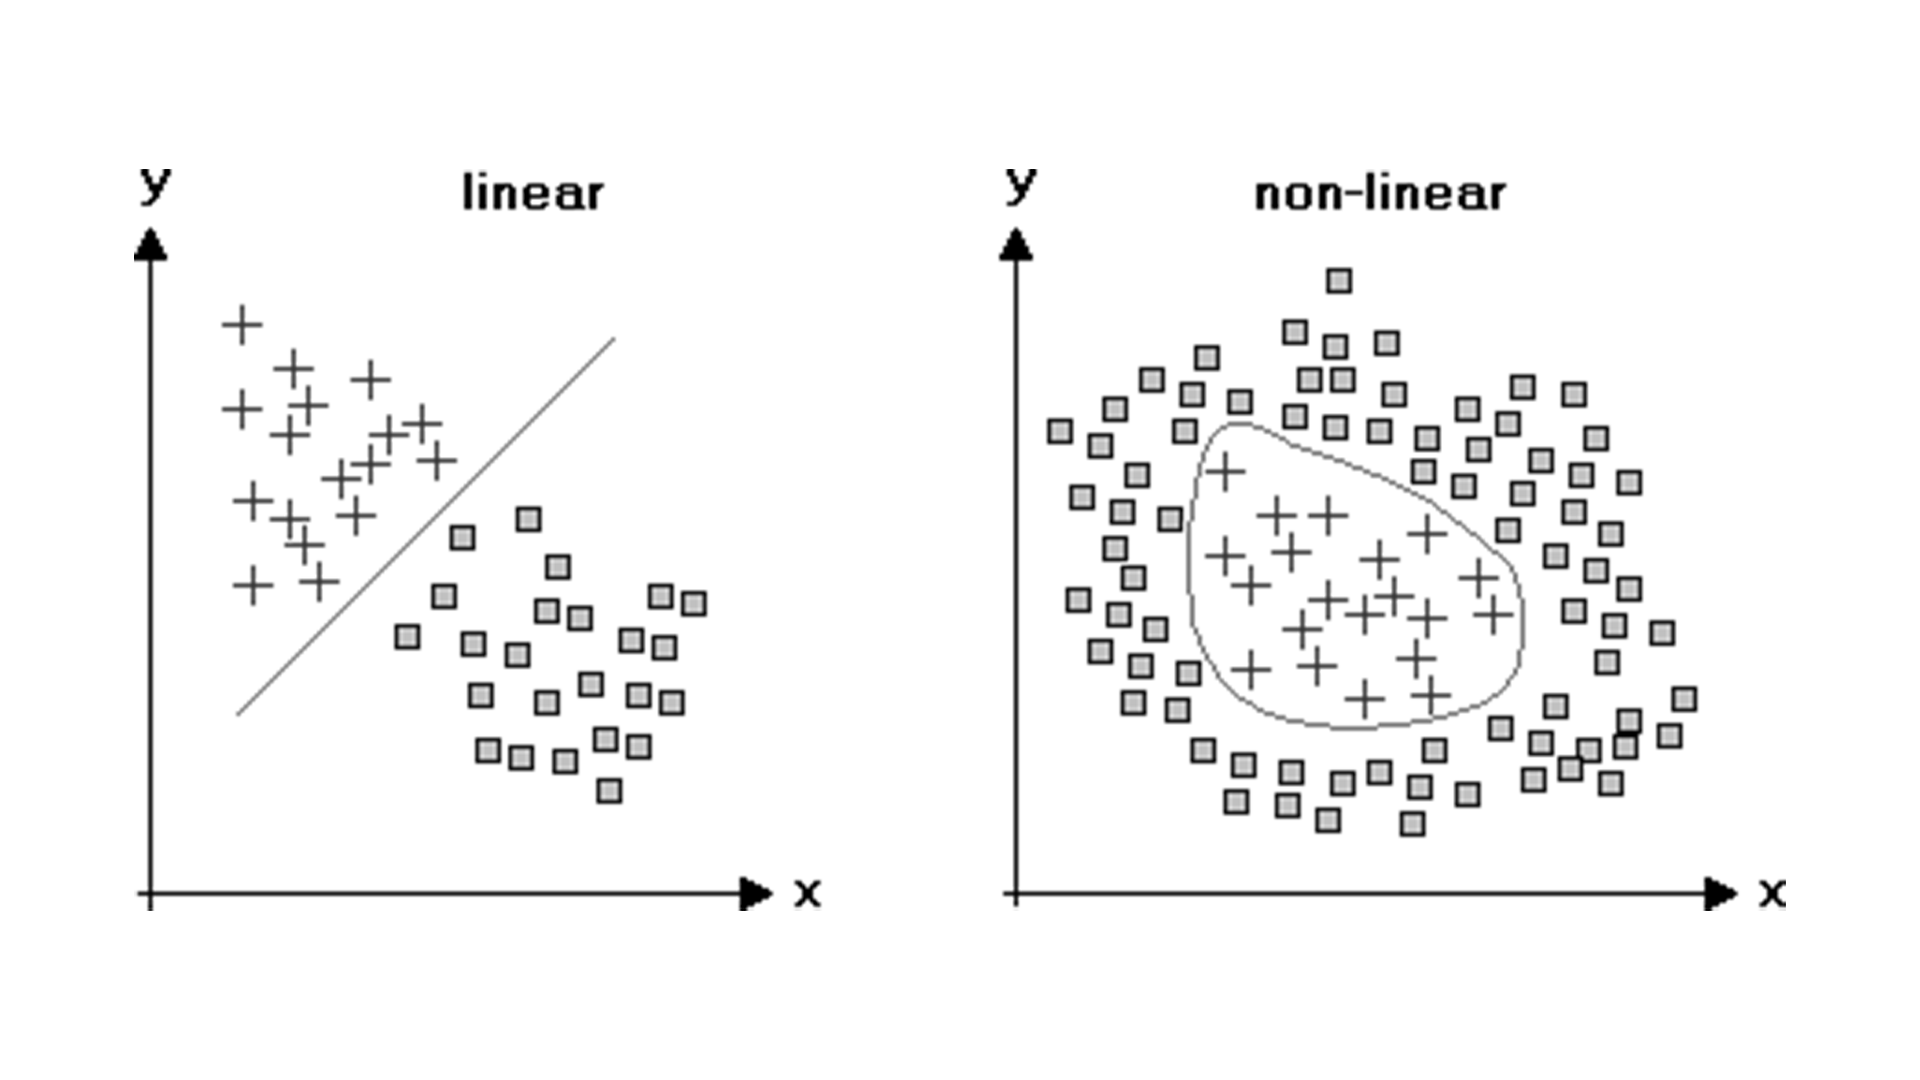
\includegraphics[width=250pt, keepaspectratio]{images/regression}
    \caption[Lineare Regression und nicht lineare Regression~\cite{6}]{Im ersten Graph ist sie gut mit der lineare Regressionen lösbar. Beim zweiten Graph ist es
    unmöglich eine genaue Regression zu bekommen mit einer lineare Regression. Dafür wird eine nicht lineare Regression verwendet~\cite{6}.}\label{regressionpic}
\end{figure}
Welche Aktivierungsfunktionen verwendet werden, kommt im Kapitel~\ref{activation} dran. So ergibt sich:
\begin{equation}
    x_{i}^{(\alpha,1)} := f^{(\alpha,1)}(\bar{x}_{i}^{(\alpha,1)}) = f^{(\alpha,1)}(\sum_{j=1}^{N_{\alpha}} w_{i,j}^{(\alpha,1)} x_{j}^{(\alpha-1,1)} + b_{i}^{(\alpha,1)}).
\end{equation}
Nun kann die Schicht auch als einen Vektor angesehen werden, wobei die Neuronen die Elemente vom Vektor sind. Folglich kann das Netzwerk
in Abbildung~\ref{fnnpic} in einem Matrixblock umgeschrieben werden~\cite{13}. So definiert sich:
\begin{equation}\label{withfunction}
    \vec{x}^{(\alpha,1)} := \begin{bmatrix}x_{1}^{(\alpha,1)} \\ x_{2}^{(\alpha,1)} \\ \ldots \\ x_{N_{\alpha}}^{(\alpha,1)} \end{bmatrix}.
\end{equation}
Sobald die letzte Schicht erreicht ist, berechnet die Verlustfunktion Fehlermaße des Netzwerkes und gibt Aussage darüber, wie gut
unsere KI ist. Mehr dazu im Kapitel~\ref{lost}.


\subsubsection{Aktivierungsfunktion}\label{activation}
Mithilfe der Aktivierungsfunktion kann die KI eine nicht lineare Regression durchführen, denn aus der Gleichung~\ref{withfunction} wird deutlich,
dass alle Operationen linear sind, wenn nur der Parameter der Funktion $f^{(\alpha,1)}(x)$ betrachtet wird. Für eine nicht lineare Regression sollte die
Aktivierungsfunktion differenzierbar sein. Dafür gibt es verschiedene Formen von Aktivierungsfunktionen, die in der Praxis angewendet werden.
Eine der meist verwendeten Aktivierungsfunktionen ist der Rectified Linear Unit (ReLU)~\cite{14}:
\begin{equation}
    f^{(\alpha,1)}(\bar{x}_{i}^{(\alpha,1)}) = \left\{
	\begin{array}{ll}
		\bar{x}_i^{(\alpha,1)}  & \mathrm{falls} \mkern5mu \bar{x}_i^{(\alpha,1)} > 0 \\
		0 & \mathrm{falls} \mkern5mu \bar{x}_i^{(\alpha,1)} \leq 0
	\end{array}
    \right..
\end{equation}
Die partielle Ableitung nach $\bar{x}_i^{(\alpha,1)}$ zur Funktion $C(\vec{y},\vec{x}^{(A,1)})$ ist:
\begin{equation}
    \frac{\partial C}{\partial \bar{x}_i^{(\alpha,1)}} = \left\{
	\begin{array}{ll}
		\frac{\partial C}{\partial {x}_i^{(\alpha,1)}}  & \mathrm{falls} \mkern5mu \bar{x}_i^{(\alpha,1)} > 0 \\
		0 & \mathrm{falls} \mkern5mu \bar{x}_i^{'(\alpha,1)} \leq 0
	\end{array}
    \right..
\end{equation}
Gründe für die Nutzung ist die Effizienz für linear gebaute Neuronale Netzwerke sowie die Berechnung der Werte. Außerdem können durch die ReLU
Neuronen dauerhaft deaktiviert werden, da alle Werte, die $\leq 0$ sind, auf $0$ gesetzt werden.
Eine weitere Aktivierungsfunktion, die für die KI verwendet wird, ist die Softmax Funktion~\cite{14}:
\begin{equation}\label{softmax}
    f^{(\alpha,1)}(\bar{x}_{i}^{(\alpha,1)}) = \frac{e^{\bar{x}_i^{(\alpha,1)}}}{\sum_{j=1}^{N_{\alpha}} e^{\bar{x}_i^{(\alpha,1)}}}.
\end{equation}
Die partielle Ableitung nach $\bar{x}_i^{(\alpha,1)}$ zur Funktion $C(\vec{y},\vec{x}^{(A,1)})$ ist:
\begin{equation}
    \frac{\partial C}{\partial \bar{x}_k^{(\alpha,1)}} = \frac{\partial C}{\partial {x}_i^{(\alpha,1)}} (\delta_{i,k}x_{i}^{(\alpha,1)}-x_{i}^{(\alpha,1)}x_{k}^{(\alpha,1)}).
\end{equation}
Meistens wird die Aktivierungsfunktion an der letzte Schicht verwendet, denn der Zweck dieser Aktivierungsfunktion ist es, mithilfe des Vektors
$ \vec{x}^{(A)} $ einen neuen Vektor gleicher Dimension zu erstellen, deren Elemente zusammenaddiert $1$ ergeben. Der Wertebereich der Funktion
liegt bei $[0;1]$. Dies kann dann in einer Wahrscheinlichkeitsverteilung dargestellt werden. Dies erleichtert die Dokumentierung der Ergebnisse der KI
und eine Rückschlussziehung, warum die KI wahrscheinlich diese Zahl nimmt, ist möglich.


\subsection{Feature Extraction}\label{feature}
Die Feature Extraction besteht aus mehreren Schichten von Operationen, mit dem das eingegebene Bild verarbeitet wird.
Eine Hauptoperation ist die 2D Convolution~\cite{15}, denn diese Operation ist dafür zuständig, dass wichtige Merkmale extrahiert werden.
Dafür werden verschiedene Filter angewendet, um verschiedene Arten von Merkmalen des Bildes zu extrahieren.
\begin{figure}[h]
    \centering
    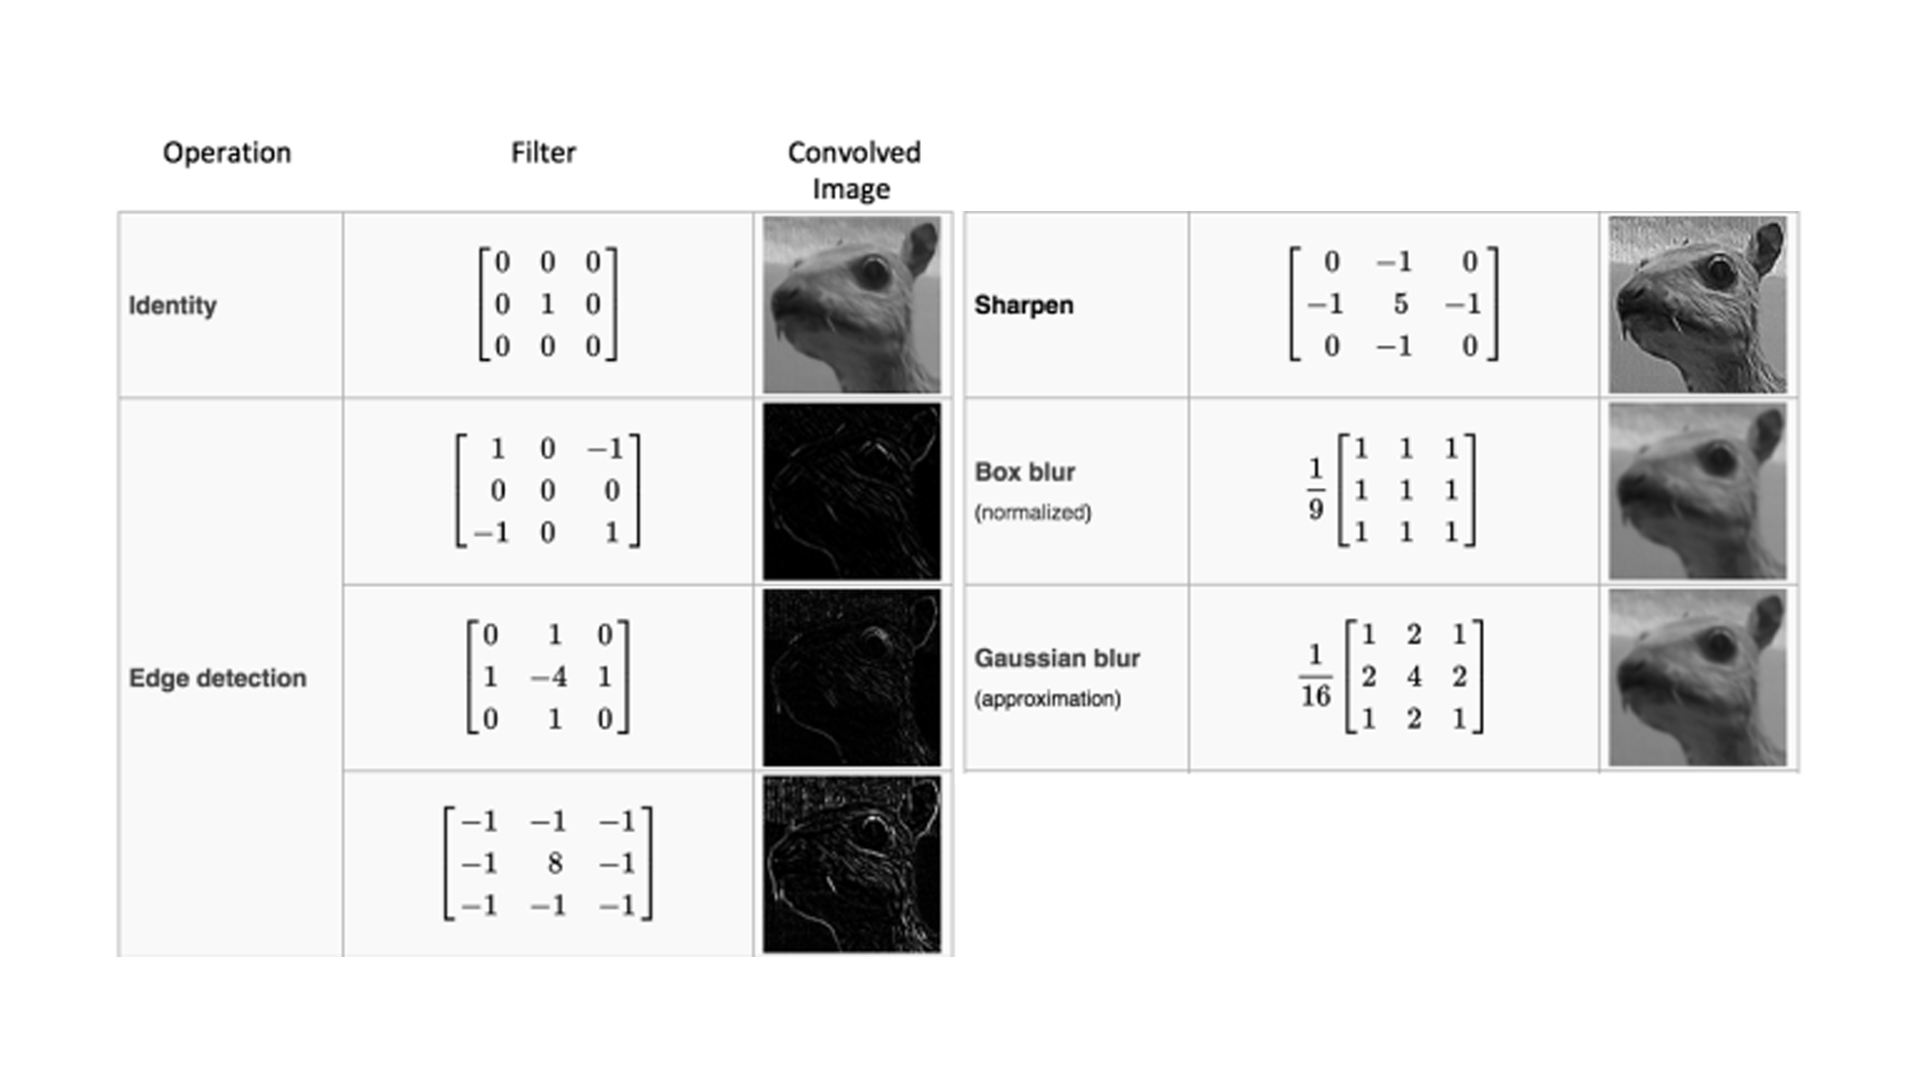
\includegraphics[width=400pt, keepaspectratio]{images/filter}
    \caption[Verschiedene Extraktionsmöglichkeiten~\cite{12}]{Hier sind verschiedene Extrahierungen zu erkennen mit verschiedenen Aufgaben. Das erste Bild mit der Operation Identity ist das Originalbild.~\cite{12}}\label{kernel}
\end{figure}
Zwei weitere wichtige Operationen sind der Max-Pooling~\cite{17} und der Flattening~\cite{18}. Aufgabe von Max-Pooling ist es, unnötige Merkmale
zu ignorieren, indem nur die hellsten Pixel rausgefiltert werden. Die Dimension des Bildes halbiert sich dadurch. Flattening ist für die Übertragung auf die Klassifikationseben zuständig,
indem die Matrix des Bildes in einen Vektor geflacht wird, sodass die KI optimal lernen kann.
Das Bild kann in einer 28\times28 Matrix dargestellt werden:
\begin{equation}
    X^{(1,1)} := (x_{ij}) \quad i \in \{1,\ldots,28\}, j \in \{1,\ldots,28\}.
\end{equation}
Der erste Index beschreibt, auf welcher Schicht die Variable sich befindet und der zweite Index beschreibt, auf welches
Bild sie sich bezieht, denn in einer Schicht können mehrere Bilder vorkommen. Dies nennt sich Tiefe. Da am Anfang aber nur ein Bild eingegeben wird, gilt
$N_{\beta}^{(1)} = 1$. Für die nächsten Schichten gilt im Allgemeinen:
\begin{equation}\label{newlayer}
    X^{(\alpha,\beta)} := (x_{ij}) \quad i \in \{1,\ldots,m_{x}^{(\alpha,\beta)}\}, j \in \{1,\ldots,n_{x}^{(\alpha,\beta)}\}.
\end{equation}
Die Werte $m_{x}^{(\alpha,\beta)}$ und $n_{x}^{(\alpha,\beta)}$ werden basierend auf der Operation berechnet, wobei
$\alpha \in \{1,\ldots,A\}$ und $\beta \in \{1^{(\alpha)},\ldots,N_{\beta}^{(\alpha)}\}$. Dabei ist die Anzahl der Tiefe von der jeweilige Schicht abhängig.


\subsubsection{2D Convolution}
Mithilfe von 2D Convolution können wichtige Merkmale herausgefiltert werden. Damit sie aber herausgefiltert werden kann, wird
eine neue Matrix definiert. Sie nennt sich Kernel:
\begin{equation}
    K^{(\alpha,\beta)}:={(k_{i,j})}^{(\alpha,\beta)} \quad i \in\{1;2;\ldots;m_{k}^{(\alpha,\beta)}\}, j \in\{1;2;\ldots;n_{k}^{(\alpha,\beta)}\}.
\end{equation}
Der Kernel kann nach der Abbildung~\ref{kernel} verschiedene Formen von Matrizen annehmen, dadurch entsteht durch die 2D Convolution eine neue Matrix, in dem Fall ein neues Bild.
Diese neue Matrix entspricht der nächsten Schicht, weshalb die neue Matrix der Gleichung~\ref{newlayer} entspricht, wobei $ m_x \leftarrow m_x - m_k + 1 $ und $ n_x \leftarrow n_x - n_k + 1 $.
Da sowohl die Eingabe des Bildes sowie der Kernel beide Matrizen sind, kann mit der 2D Convolution gerechnet werden. Sie ist
folgendermaßen definiert~\cite{16}:
\begin{equation}
    a_{i,j} = {(X \ast K)}_{i,j} := \sum_{m'=1}^{m_{k}} \sum_{n'=1}^{n_{k}} x_{i-m'+1,j-n'+1}k_{m',n'}. \label{Conv}
\end{equation}
Eine weitere Operation, die sehr wichtig für die 2D Convolution ist, ist die Kreuzkorrelation (Cross Correlation)~\cite{16}:
\begin{equation}
    a_{i,j} = {(X \star K)}_{i,j} := \sum_{m'=1}^{m_{k}} \sum_{n'=1}^{n_{k}} x_{i+m'-1,j+n'-1}k_{m',n'}.
\end{equation}
Aus~\eqref{Conv} wird deutlich, dass Cross Correlation nichts anderes ist als eine 2D Convolution, wo nur der Kernel um 180$^{\circ}$
rotiert wird. Für die Operation können auch Biases sowie Aktivierungsfunktionen angewandt werden. Dies ähnelt der Struktur der FNN.\@
Werden diese Eigenschaften hinzugefügt, folgt daraus für die 2D Convolution:
\begin{equation}
    x_{i,j}^{(\alpha,\beta)} = f^{(\alpha)}(\sum_{\beta'=1}^{N_{\beta}^{(\alpha-1)}} \sum_{m'=1}^{m_{k}} \sum_{n'=1}^{n_{k}} x_{i+m'-1,j+n'-1}^{(\alpha-1,\beta')}k_{m',n'}^{(\alpha,\beta')}+b_{i,j}^{(\alpha,\beta)}).
\end{equation}
Für die Backpropagation werden die partiellen Ableitungen nach $k_{i,j}^{(\alpha,\beta)}$, nach $b_{i,j}^{(\alpha,\beta)}$ und nach $x_{i,j}^{(\alpha-1,\beta)}$ zur Funktion $C$ gebraucht~\cite{16}:
\begin{equation}
    \frac{\partial C}{\partial k_{i,j}^{(\alpha,\beta)}} = \sum_{i'=1}^{m_x^{(\alpha,\beta)}}\sum_{j'=1}^{n_x^{(\alpha,\beta)}} \frac{\partial C}{\partial \bar{x}_{i',j'}^{(\alpha,\beta)}}
    x_{i+i'-1,j+j'-1}^{(\alpha-1,\beta)} = {(X^{(\alpha-1,\beta)} \star \frac{\partial C}{\partial \bar{X}^{(\alpha,\beta)}})}_{i,j},
\end{equation}
\begin{equation}
    \frac{\partial C}{\partial b_{i,j}^{(\alpha,\beta)}} = \frac{\partial C}{\partial \bar{x}_{i,j}^{(\alpha,\beta)}},
\end{equation}
\begin{equation}
    \frac{\partial C}{\partial x_{i,j}^{(\alpha-1,\beta)}} = \sum_{i'=1}^{m_x^{(\alpha,\beta)}}\sum_{j'=1}^{n_x^{(\alpha,\beta)}} \frac{\partial C}{\partial \bar{x}_{i',j'}^{(\alpha,\beta)}} k_{i-i'+1,j-j'+1}^{(\alpha,\beta)}
    = {(K^{(\alpha,\beta)} \ast \frac{\partial C}{\partial \bar{X}^{(\alpha,\beta)}})}_{i,j}.
\end{equation}

\subsubsection{Max-Pooling}
Diese Operationen werden für das CNN öfters benutzt, denn zum einen reduziert sie Bildgröße um die Hälfte und zum anderen behält sie trotzdem wichtige
Merkmale des Bildes. Das macht die Berechnungen nochmal effizienter und die Hauptmerkmale werden hervorgehoben. Dies funktioniert, indem eine 2$\times$2 Matrix
durch die einzelnen Regionen des Bildes schrittweise berechnet werden und der höchste Wert von den 4 Pixel ausgewählt wird~\cite{17}:
\begin{equation}
    x_{i,j}^{(\alpha,\beta)} = \max\{x_{i',j'}^{(\alpha-1,\beta)},x_{i',j'+1}^{(\alpha-1,\beta)},x_{i'+1,j'}^{(\alpha-1,\beta)},x_{i'+1,j'+1}^{(\alpha-1,\beta)}\},
\end{equation}
wobei $i' = 2i-1$ und $j' = 2j-1$ gilt. Die neue Dimension beträgt:
\begin{equation}
    m_{x}^{(\alpha,\beta)} = \bigg\lceil \frac{m_{x}^{(\alpha-1,\beta)}}{2} \bigg\rceil, \mkern5mu
    n_{x}^{(\alpha,\beta)} = \bigg\lceil \frac{n_{x}^{(\alpha-1,\beta)}}{2} \bigg\rceil.
\end{equation}
Bei der Backpropagation ist der Wert der Verlustfunktion nur von den größten Werten der einzelnen Regionen abhängig, da nur diese an die nächste Schicht weitergegeben wurde.
Die anderen Werte spielen keine Rolle, deswegen ist der Gradient von denen = 0:
\begin{equation}
    \frac{\partial C}{\partial x_{i,j}^{(\alpha-1,\beta)}} =
    \left\{
    \begin{array}{ll}
		\frac{\partial C}{\partial \bar{x}_{i,j}^{(\alpha,\beta)}} & \mathrm{falls} \mkern5mu \max\{x_{i,j}^{(\alpha-1,\beta)},x_{i,j+j'}^{(\alpha-1,\beta)},x_{i+i',j}^{(\alpha-1,\beta)},x_{i+i',j+j'}^{(\alpha-1,\beta)}\} \\
		0 & \mathrm{falls} \mkern9mu \mathrm{Sonstiges}
	\end{array}
    \right.,
\end{equation}
dabei gilt für $i'$ und $j'$:
\begin{equation}
i' =
    \left\{
    \begin{array}{ll}
		1 & \mathrm{falls} \mkern5mu 2 \mid i\\
		-1 & \mathrm{falls} \mkern9mu 2 \nmid i
	\end{array}
    \right.,
\end{equation}
\begin{equation}
    j' =
        \left\{
        \begin{array}{ll}
            1 & \mathrm{falls} \mkern5mu 2 \mid j\\
            -1 & \mathrm{falls} \mkern9mu 2 \nmid j
        \end{array}
        \right..
    \end{equation}

\subsubsection{Übergang von Feature Extraction zu Klassifikationsebene}
Nachdem die Merkmale der Bilder durch 2D Convolution und Max-Pooling extrahiert wurden, muss diese Matrix zur Klassifikationsebene übertragen werden.
Da aber die Klassifikationsebene nur einen Vektor als Eingabe annimmt, muss die Matrix abgeflacht werden. Mithilfe des Vektoroperators $vec()$ kann die
Ausgangsmatrix der Feature Extraction in einen Vektor umgewandelt werden:
\begin{equation}
    \vec{x}^{(\alpha,\beta)} = vec_{n_{x}^{(\alpha,\beta)}, m_{x}^{(\alpha,\beta)}}(X^{(\alpha-1,\beta)T}).
\end{equation}
Dabei geben die Indizes die Dimension der Matrix an, die abgeflacht werden soll. Für die Backpropagation muss der Vektor aber wieder in eine Matrix mit
der gleichen Dimension umgeformt werden. Dafür existiert eine Umkehrfunktion des Vektoroperators $vec^{-1}()$ die diese Berechnung durchführen kann:
\begin{equation}
    X^{(\alpha-1,\beta)} = vec^{-1}_{n_{x}^{(\alpha,\beta)}, m_{x}^{(\alpha,\beta)}}{(\vec{x}^{(\alpha,\beta)})}^{T}.
\end{equation}
Dieser Übergang wird auch Flattening genannt~\cite{18}.

\subsection{Verlustfunktion}\label{lost}
Um auszuwerten, ob eine KI gute oder schlechte Vorhersagen trifft, werden Verlustfunktionen verwendet.
Verlustfunktionen sind Funktionen, die die Abweichung der vorhergesagten Zahl $\vec{x}^{(A,1)}$ von der Ausganszahl $\vec{y}$ berechnen.
Je größer die Abweichung ist, desto unpräziser ist die Vorhersage. Für die
Optimierung bedeutet dies, dass der Wert der Verlustfunktion kleinstmöglich wird, sodass die KI präzise Vorhersagen treffen kann. Durch die Änderung der Parameter
kann die Verlustfunktion minimiert werden, denn die Verlustfunktion ist von allen Parameter $w$,$b$ und $k$ in der Variable $\vec{x}^{(A,1)}$ abhängig.
Es gilt:
\begin{equation}
    C(\vec{y},\vec{x}^{(A,1)}) \equiv C(\vec{y},\vec{w},\vec{b},\vec{k}),
\end{equation}
 wobei $N_w$ die Gesamtanzahl der Gewichte, $N_b$ die Gesamtanzahl der Bias und $N_k$ die Gesamtanzahl der Kernels sind:
\begin{equation}
    \vec{w} := \begin{bmatrix} w_{1} \\ w_{2} \\ \ldots \\ w_{N_w} \end{bmatrix},
    \vec{b} := \begin{bmatrix} b_{1} \\ b_{2} \\ \ldots \\ b_{N_b} \end{bmatrix},
    \vec{k} := \begin{bmatrix} k_{1} \\ k_{2} \\ \ldots \\ k_{N_k} \end{bmatrix}.
\end{equation}
Doch wie die Parameter richtig gesetzt werden, kommt in Kapitel
~\ref{gradient} dran.\@ Im Folgendem wird die Kreuzentropie (Cross Entropy) verwendet~\cite{19}. Sie ist folgendermaßen definiert:
\begin{equation}
    C(\vec{y},\vec{x}^{(A,1)}) = -\sum_{i=1}^{N_A} y_i \ln(x_i^{(A,1)}).
\end{equation}
Die folgende partielle Ableitung nach $x_i^{(A,1)}$ ist:
\begin{equation}
    \frac{\partial C}{\partial x_i^{(A,1)}} = -\frac{y_i}{x_i^{(A,1)}}.
\end{equation}
Voraussetzung der Cross Entropy ist, dass $\sum_{i=1}^{N_A} x_i^{(A,1)} = 1$ ergibt und dass die KI auf einer Klassifizierung basiert. Dies wird durch die Softmax Funktion in der Gleichung~\ref{softmax} erfüllt.
Vorteil dieser Verlustfunktion ist zum einen, dass sie die Abweichung präzise für die Wahrscheinlichkeitsverteilung berechnen kann.

\subsection{Optimierung}\label{gradient}
Mithilfe der Optimierung kann die Abweichung der Verlustfunktion verringert werden, indem die Parameter optimal gewählt werden. In der Analysis
wird die erste Ableitung der Verlustfunktion genommen und auf $0$ gesetzt. Problem bei der Rechnung ist nun, dass in der Praxis die Anzahl der Parameter
der KI sehr hoch sein kann. Es wird von mehreren Tausenden Parametern gesprochen. So ist die Berechnung der Parameter uneffizient und könnte für einen
Rechner sehr lange dauern, bis sie perfekte Parameter für die Verlustfunktion findet. Deswegen werden auf Algorithmen zurückgegriffen, die diese
Berechnungen deutlich zeitsparender durchführen können. Einer dieser Algorithmen nennt sich Gradientenverfahren. Das Gradientenverfahren besagt, dass die höchste
Steigung, die zurückgelegt werden kann, mit einen $\nabla C$ definiert wird~\cite{5}:
\begin{equation}\label{gradientdefinition}
    \nabla C =
    \begin{bmatrix}
        \frac{\partial C}{\partial y_{1}} & \frac{\partial C}{\partial w_{1}} & \frac{\partial C}{\partial b_{1}} & \frac{\partial C}{\partial k_{1}}
        \\ \frac{\partial C}{\partial y_{2}} & \frac{\partial C}{\partial w_{2}} & \frac{\partial C}{\partial b_{2}} & \frac{\partial C}{\partial k_{2}}
        \\ \cdots & \cdots & \cdots & \cdots
        \\ \frac{\partial C}{\partial y_{N_y}} & \frac{\partial C}{\partial w_{N_w}} & \frac{\partial C}{\partial b_{N_b}} & \frac{\partial C}{\partial k_{N_k}}
    \end{bmatrix}.
\end{equation}
Da aber das Minimum der Funktion gesucht wird, wird die tiefste Steigung
benötigt, indem $\nabla C$ negativ wird, also $-\nabla C$. Aus der Gleichung~\ref{gradientdefinition} können die Elemente für die Annäherung der optimalen Parameter genutzt werden.
So kann durch jede Iteration, der Parameter aktualisiert werden~\cite{8}:
\begin{equation}
    w_i \leftarrow w_i - \Delta w_i \equiv  w_i - \eta \frac{\partial C}{\partial w_{i}},
\end{equation}
\begin{equation}
    b_i \leftarrow b_i - \Delta b_i \equiv  b_i - \eta \frac{\partial C}{\partial b_{i}},
\end{equation}
\begin{equation}
    k_i \leftarrow k_i - \Delta k_i \equiv  k_i - \eta \frac{\partial C}{\partial k_{i}}.
\end{equation}
Hier wurde ein neuer Parameter $\eta$ hinzugefügt, dieser nennt sich Lernrate. Die Lernrate gibt an, wie schnell sie sich an das Minimum antasten soll.
Es ist wichtig, einen guten Wert für die Lernrate zu setzen, denn falls sie zu groß wird, kann sie vielleicht über das Minimum vorbeispringen.
Wenn aber die Lernrate zu klein ist, dann dauert auch das Lernen deutlich länger, da die Optimierung langsamer am Minimum antastet.
\begin{figure}[h]
    \centering
    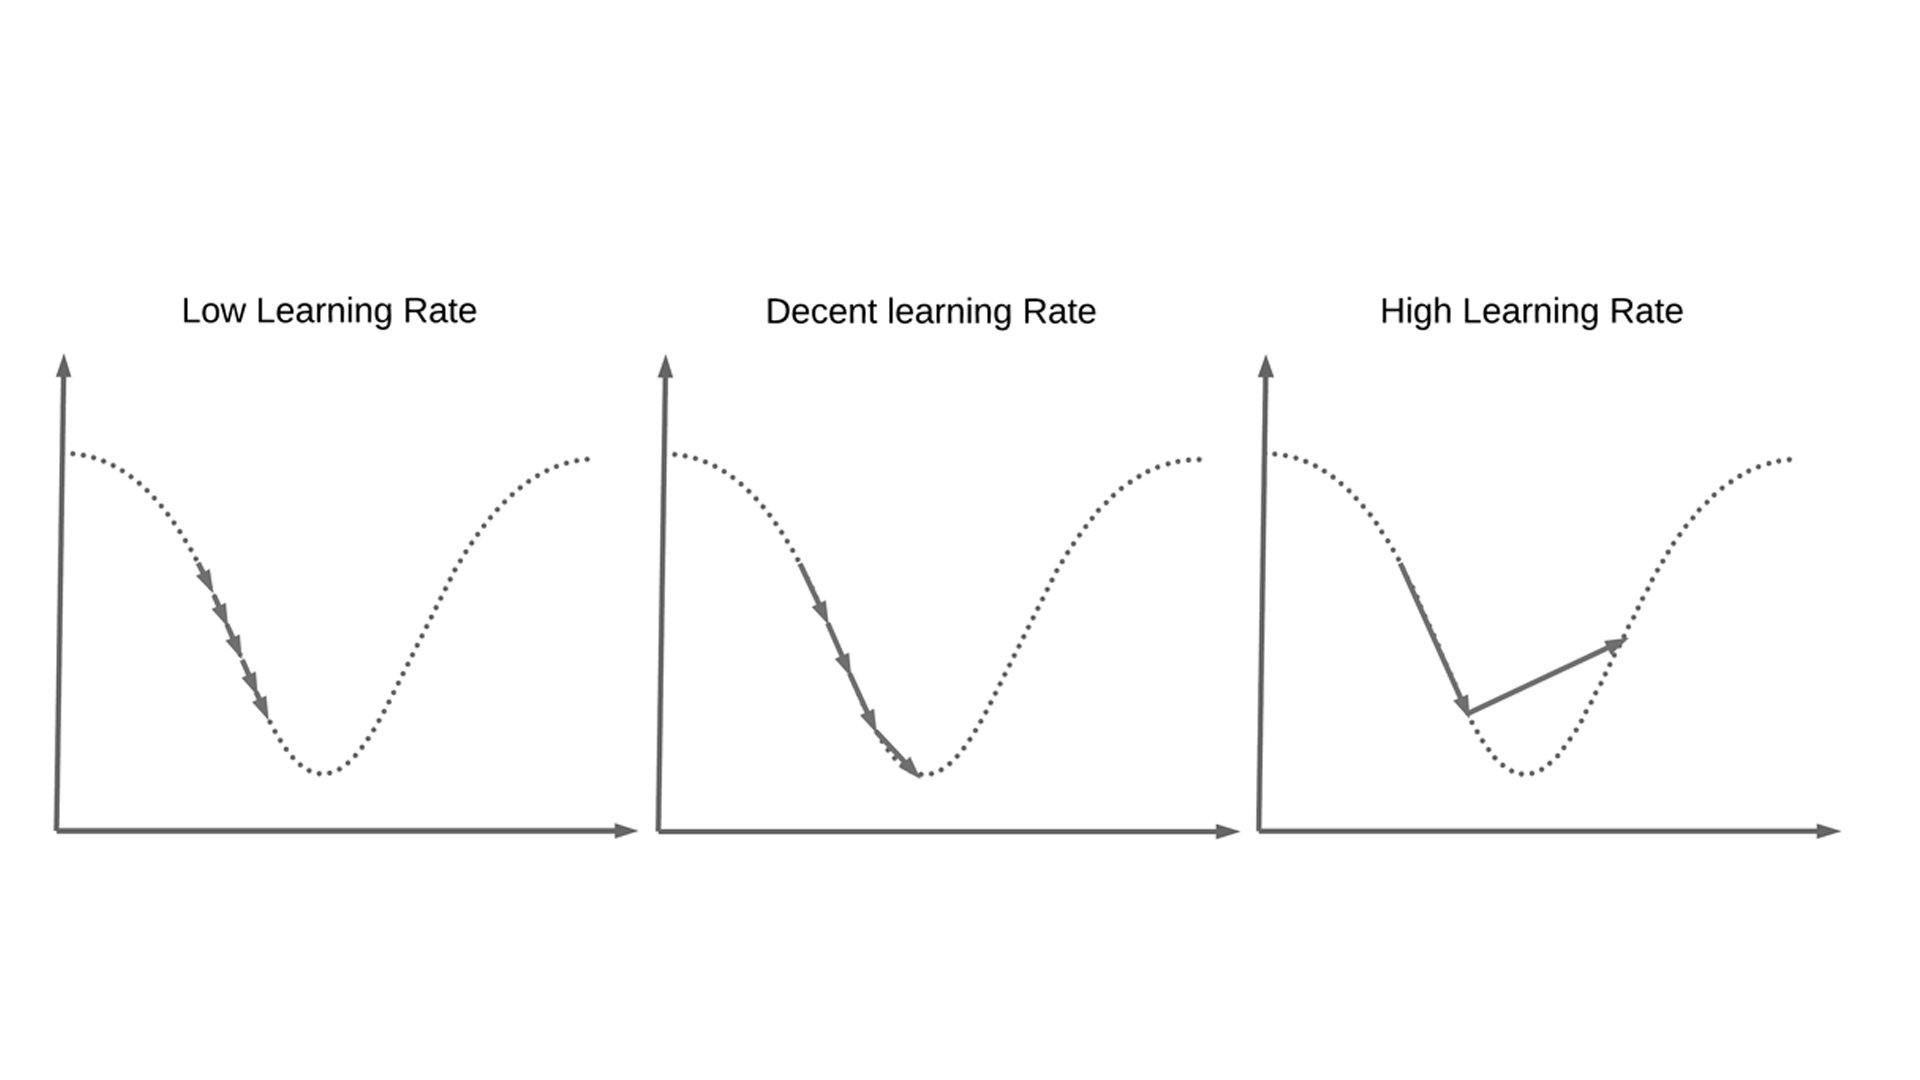
\includegraphics[width=300pt, keepaspectratio]{images/lrate}
    \caption[Einstellen der Lernrate~\cite{22}]{Sehr gut erkennbar sind die Iterationen: Wenn die Lernrate richtig gewählt ist, dann erreicht sie das Minimun schneller.~\cite{22}}
\end{figure}
Trotz des Algorithmus kann die Berechnung immer noch nicht effizient genug sein, denn wenn als
Beispiel der Datensatz von MNIST verwendet wird, dann müssen für alle 70000 Bilder die Gradienten berechnet werden. Diese Zeit kann reduziert werden,
indem nicht für alle Bilder der Gradient berechnen werden müssen. Als Beispiel soll nur der Gradient für jedes 100. Bild berechnet werden. So werden anstatt
für 70000 Bilder, die Gradienten von nur 700 Bilder berechnet. Das Antasten des Minimums ist nicht sehr präzise, aber dennoch aussagekräftig und zeitsparend. Die
Optimierung nennt sich Stochastisches Gradientenverfahren (SGD)~\cite{8}.
\subsubsection{Backpropagation}\label{back}
Um die Parameter zu aktualisieren, muss der Wert $\frac{\partial C}{\partial w_{i}}$ berechnet werden. Mithilfe der Backpropagation kann dieser Wert
berechnet werden, indem rückwärts gegangen wird vom FNN.\@ Als Beispiel wird ein FNN dargestellt mit drei Schichten. Für die Verlustfunktion soll der
Cross Entropy verwendet werden. Ziel ist es, den Parameter $w_{2,3}^{(2,1)}$ zu aktualisieren, weshalb $\frac{\partial C}{\partial w_{2,3}^{(2,1)}}$ gesucht ist.
\begin{figure}[h]
    \centering
    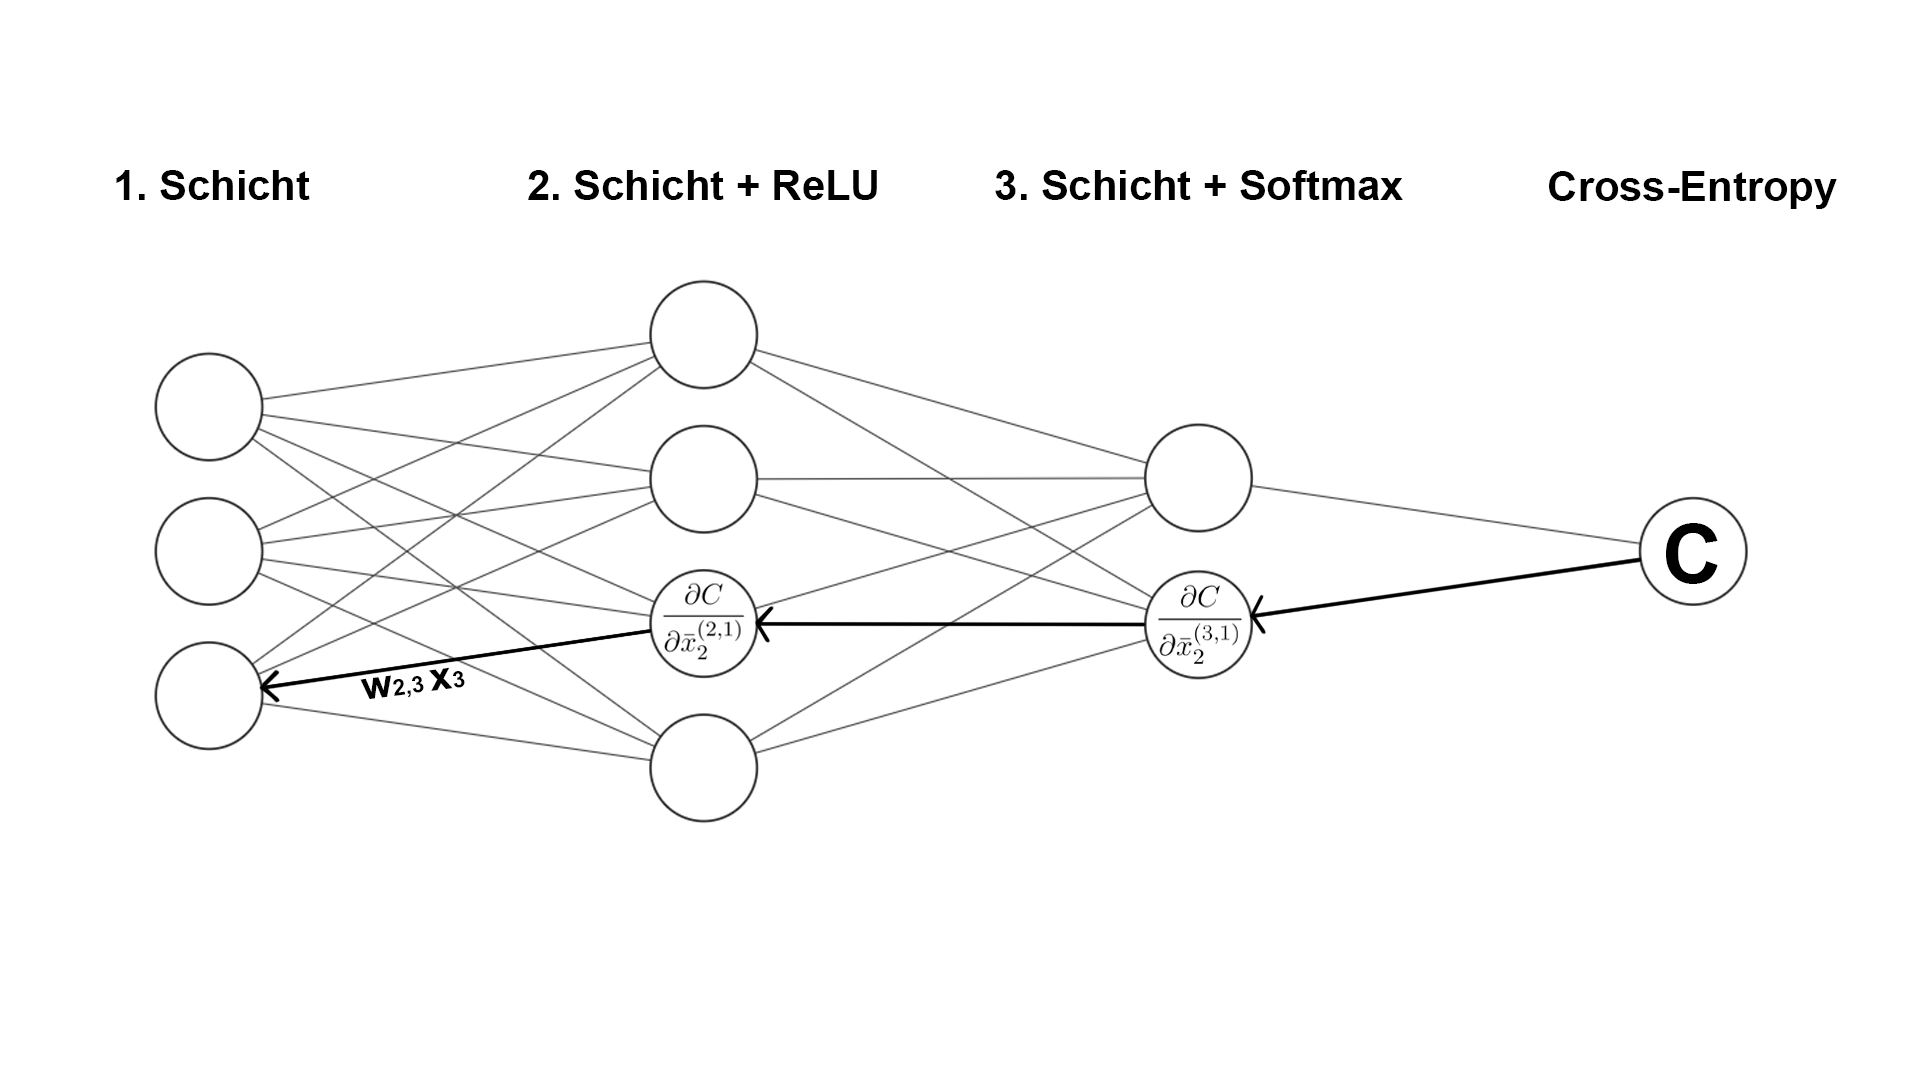
\includegraphics[width=400pt, keepaspectratio]{images/beispiel}
    \caption[Beispiel eines FNNs]{Der Pfad von der Verlustfunktion zum Parameter $w_{2,3}^{(2,1)}$. Dafür wird die Kettenregel angewendet, um die Abhängigkeit von $w_{2,3}^{(2,1)}$ zu berechnen.}
\end{figure}
Dafür wird angeschaut, wie die Verlustfunktion $C$ von $w_{2,3}^{(2,1)}$ abhängt.
Da die Werte bei jeder Schicht weitergegeben wurden, kann die Kettenregel angewendet werden~\cite{5}:
\begin{equation}
    \frac{\partial C}{\partial w_{2,3}^{(2,1)}} = \frac{\partial C}{\partial x_2^{(3,1)}} \frac{\partial x_2^{(3,1)}}{\partial \bar{x}_2^{(3,1)}}
    \frac{\partial \bar{x}_2^{(3,1)}}{\partial x_2^{(2,1)}} \frac{\partial x_2^{(2,1)}}{\partial \bar{x}_2^{(2,1)}}
    \frac{\partial \bar{x}_2^{(2,1)}}{\partial w_{2,3}^{(2,1)}}.
\end{equation}
Dies kann abgekürzt werden mit:
\begin{equation}\label{einfacher}
    \frac{\partial C}{\partial w_{2,3}^{(2,1)}} = \frac{\partial C}{\partial \bar{x}_2^{(2,1)}} \frac{\partial \bar{x}_2^{(2,1)}}{\partial w_{2,3}^{(2,1)}} \stackrel{(\ref{w})}{=} \frac{\partial C}{\partial \bar{x}_2^{(2,1)}} x_3^{(1,1)}.
\end{equation}
Die Gleichung~\ref{einfacher} ist für die Umsetzung deutlich angenehmer, da der Wert $\frac{\partial C}{\partial \bar{x}_2^{(2,1)}}$ von der nächsten Schicht
schon berechnet wurde. Dies bedeutet, dass nur der Wert $\frac{\partial \bar{x}_2^{(2,1)}}{\partial w_{2,3}^{(2,1)}}$ berechnet werden muss.

\section{Umsetzung}
Zuerst braucht es eine Struktur für das CNN.\@ Dafür wird eine Klasse Layer erstellt, die als Objekt angesehen werden soll. Dabei soll die Klasse Layer folgende
Eigenschaften besitzen: Eine Eingabe und eine Ausgabe. Außerdem wird eine neue Klasse DenseLayer erstellt, die diese Eigenschaften der Klasse Layer erbt.
Der DenseLayer soll die Schichten im FNN darstellen und die Parameter $w$ und $b$ als Variablen annehmen können. Weitere Klassen, wie Schichten für die
Feature Extraction oder Aktivierungsfunktion und Verlustfunktion müssen erstellt werden. Vorteil an der Programmierung sind die Open Source Pakete, die das
Internet anbietet. So müssen nicht die einzelnen Elemente der Vektoren ausgerechnet werden, sondern es lassen sich alle Elemente des Vektors auf einmal berechnen.
Auch muss der Lernprozess programmiert werden, indem das Netzwerk durchlaufen wird. Die Anzahl der Durchläufe des Netzwerkes kann bestimmt werden.
Diese nennt sich auch Epochen. Am Ende werden verschiedene Diagramme generiert, die für die Analyse der KI nützlich sein könnten.
Mehr dazu im Kapitel~\ref{auswertung}. Für die Architektur des Netzwerkes werden mehrere Schichten von 2D Convolution sowie Schichten von Max Pooling angesetzt.
Der Aufbau ist gut im Abbild 12 zu erkennen.
\begin{figure}[h]
    \centering
    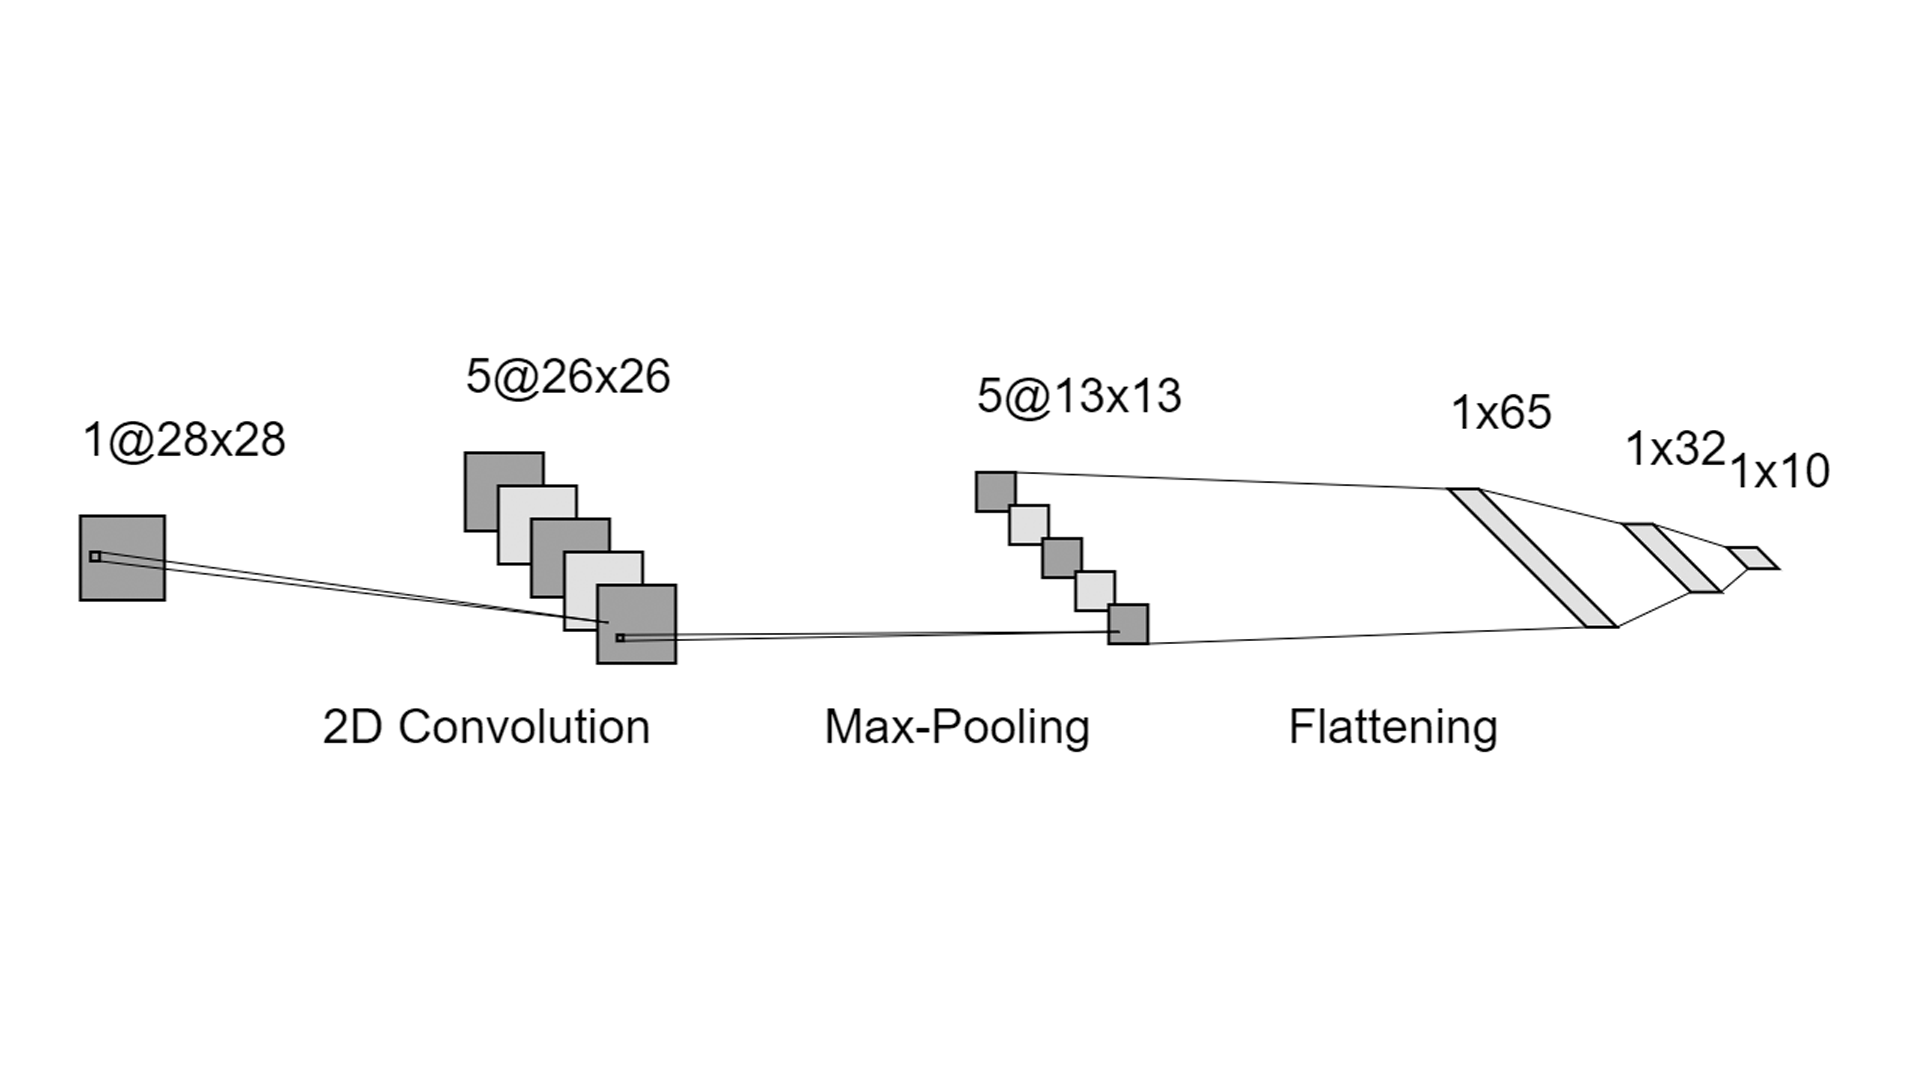
\includegraphics[width=325pt, keepaspectratio]{images/cnn}
    \caption[Architektur eines CNNs]{Insgesamt 8 Schichten mit gestapelten Operationen, wie die 2D Convolution, oder der Max Pooling.
    Die Anzahl der Ausgabeschicht liegt bei 10, für die einzelnen Ziffern von 0-9.}
\end{figure}
Nach der Max-Pooling Schicht wird das zum Vektor abgeflacht und mit zwei weiteren neuronalen Schichten verbaut.
Mit dem Netzwerk wird die Facharbeit die KI trainieren.

\subsection{Werkzeuge}
Für die Umsetzung wird die Programmiersprache Python verwendet, denn Python wird in der Praxis größtenteils im Bereich Data Science verwendet~\cite{20}.
Python wird dafür verwendet, weil es im Gegensatz zu anderen Programmiersprachen viele Open Source Pakete besitzt.
Denn Python ist im Jahr 2023 die meist genutzte Programmiersprache~\cite{21}. Dabei spielen zwei Pakete eine wichtige Rolle für die Umsetzung:
NumPy und Matplotlib. NumPy ist ein Paket für Vektor- und Matrizenberechnungen und berechnet die Werte effizienter als Python selbst. Außerdem
bietet sie sehr viele Operationen an, die für die KI notwendig sind. Der Matplotlib ist für die Visualisierung der Bilder sowie die Filter von der
Feature Extraction zuständig. Sie hilft den Nutzer, die KI besser zu verstehen und nachzuvollziehen.

\subsection{Trainingsphase}
Bevor der Ablauf in der Trainingsphase erklärt wird, wird der Datensatz in 3 Teilen aufgespalten: Die Trainingsdaten, die Validierungsdaten
und die Testdaten. Das Verhältnis der Verteilung kann unterschiedlich sein. Meistens sind sie in 50/30/20 aufgeteilt.
Für die Trainingsphase werden erst mal nur die Trainingsdaten und die Validierungsdaten verwendet.
Bevor die Trainingsphase gestartet wird, werden für alle verstellbare Parameter $w$, $b$ und $k$ zufällige Werte über
die Gauß-Verteilung gegeben. Zuerst wird ein zufälliges erstes Bild aus den Trainingsdaten in die Eingabeschicht weitergeleitet.
Bis zur Ausgabeschicht berechnet die KI die entsprechende Vorhersage. Mit der Vorhersage wird die Fehlerabweichung mit dem richtigen
Ergebnis mithilfe der Verlustfunktion berechnet. Die Parameter werden dann durch den SGD optimiert mithilfe von Backpropagation.
Danach wird das nächste zufällige Bild ausgewählt und die Schritte werden wiederholt. Dies gilt so lange, bis alle Bilder aus
den Trainingsdaten einmal vorgekommen sind. Zuletzt werden die Bilder aus den Validierungsdaten
in die Eingabeschicht weitergeleitet und die KI soll die Zahl vorhersagen. Der Unterschied ist aber, dass die Parameter nicht optimiert werden
und dass sozusagen die KI nur getestet wird. Die erste Epoche endet somit und die zweite Epoche beginnt. Sie wiederholt die oben genannten Schritte,
wie in der ersten Epoche. Der Vorteil ist aber, dass sie mit den verbesserten Parameter weiterrechnet. Die Anzahl der Epochen, die durchgangen
werden sollen, kann selber bestimmt werden. Für die Facharbeit wurde die Epoche auf 200 gesetzt. Am Ende der Trainingsphase wird ein Diagramm
angezeigt, die für das Kapitel Auswertung eine wichtige Rolle spielen.

\subsection{Auswertung}\label{auswertung}
Manchmal kann eine schlecht ausgewählte Struktur des Netzwerkes die Vorhersehbarkeit der KI beeinträchtigen.
Dafür werden zwei neue Begriffe definiert: Überfittung (Overfitting) und Unterfittung (Underfitting)~\cite{7}.
Als Beispiel werden 3 verschiedene Regressionen verwendet:
\begin{figure}[h]
    \centering
    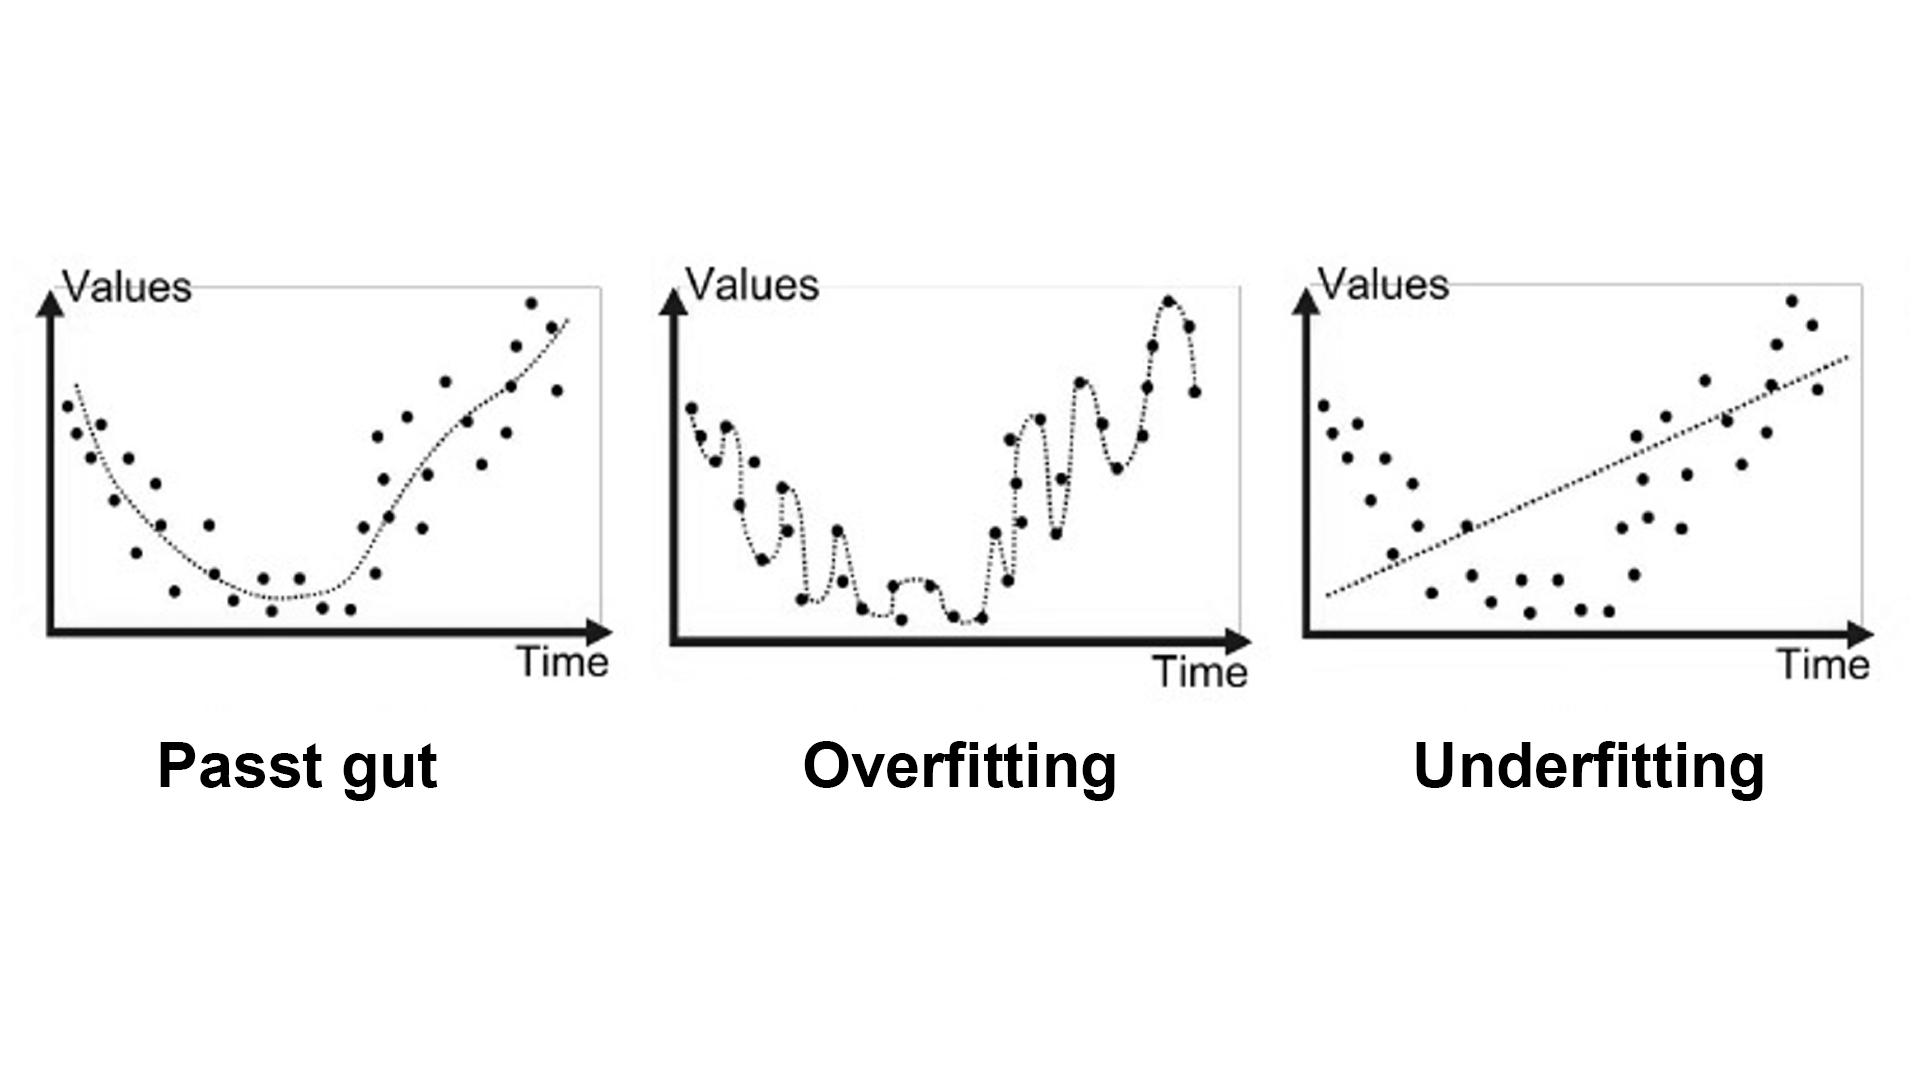
\includegraphics[width=300pt, keepaspectratio]{images/overfitting}
    \caption[Overfitting und Underfitting~\cite{7}]{Die Regressionen werden als Beispiel mit Overfitting und Underfitting dargestellt~\cite{7}.}
\end{figure}
Von den 3 Regressionen ist die erste Regression gut gewählt, denn sie verläuft nicht allzu perfekt in den Punkten. Trotzdem sind die
Abweichungen gering. Bei der zweiten Regression wird Overfitting erkannt, denn sie verläuft zu perfekt in den Punkten, doch wenn
ein neuer unbekannter Punkt eingefügt wird, dann kann die Regression zu falsche Ergebnisse führen. Das Gegenteil davon ist Underfitting
bei der dritten Regression. Hier wird deutlich gezeigt, dass die Abweichungen zu hoch sind, weil die Regression linear ist.
Dies kann mit der Trainingsphase bei der KI übertragen werden, denn die KI soll sich nicht zu sehr auf die Trainingsdaten gewöhnen,
sondern auch von unbekannten Daten gut vorhersagen. Deswegen spielen die Validierungsdaten eine wichtige Rolle, um gegen Overfitting
und Underfitting vorzugehen. Um zu sagen, wie gut eine KI vorhersagen kann, werden sogenannte Metriken verwendet. Metriken sind Bewertungskriterien für die KI,
wie gut sie vorhersagen kann. Eine, die für die Facharbeit genommen wird, ist die Genauigkeit (Accuracy)~\cite{21}. Sie lässt sich folgendermaßen
berechnen:
\begin{equation}
    \text{Accuracy} = \frac{\text{Anzahl der richtig vorhergesagten Bildern}}{\text{Anzahl der Gesamtbildern}}.
\end{equation}
Das Diagramm, das in Kapitel Trainingsphase erwähnt wurde, ist ein Epoche-Accuracy Diagramm und sieht folgendermaßen aus, nachdem die Trainingsphase
beendet wurde:
\begin{figure}[h]
    \centering
    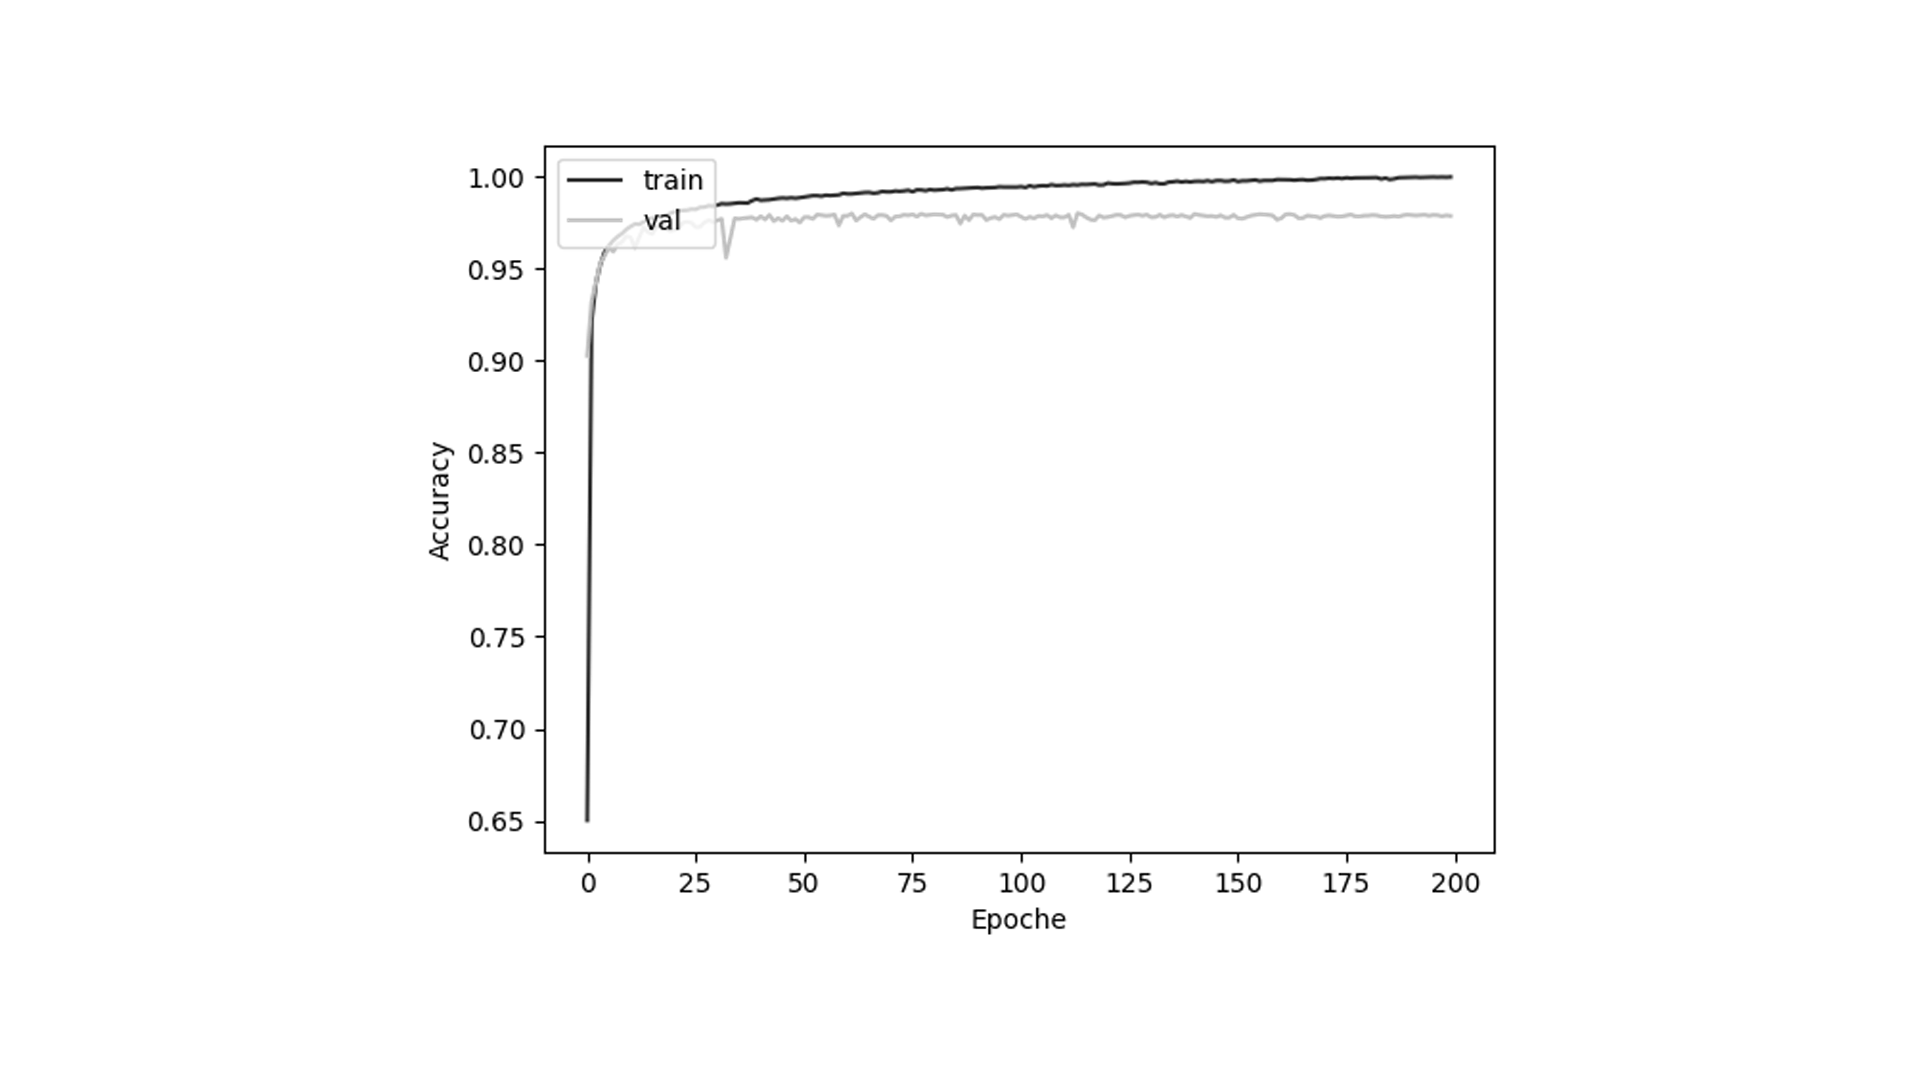
\includegraphics[width=375pt, keepaspectratio]{images/accuracydiagram}
    \caption[Epoche-Accuracy Diagramm]{Epoche-Accuracy Diagramm mit den Werten der Testdaten und der Validierungsdaten. Der Abstand vergrößert sich,
    die KI fängt an zu überfitten.}
\end{figure}
Hier ist gut zu sehen, dass während die Accuracy der Trainingsdaten nach oben steigt, die Validierungsdaten der KI konstant bleibt. Der Abstand zwischen den
beiden Werten nimmt zu. Dies deutet auf Overfitting hin und kann durch frühzeitiges Aufhören verhindert werden. Für diesen Fall reichen
75 Epochen. Zum Schluss werden die Testdaten auch in das Netzwerk eingeschickt und versucht vorherzusagen. Unterschied zwischen den Validierungsdaten
und Testdaten ist, dass die Testdaten noch keinen Kontakt mit der KI hatten, sodass die KI getestet werden kann.
Nach der Durchführung liegt der Accuracy Wert der Testdaten bei 98,17\%~\cite{9}.

\section{Schlussfolgerung}
Die folgende Facharbeit ging der Leitfrage nach, wie eine handgeschriebene Zahl mithilfe einer KI erkannt werden. Dazu wurde eine KI umgesetzt, die diese Problemstellung lösen kann.
Am Ende hat sich herausgegeben, dass die KI mit einer Wahrscheinlichkeit von 98,17\% die handgeschriebene Zahl erkennen konnte. Diese Umsetzung ist mithilfe der Mathematik, wie
eine KI funktioniert und wie sie aufgebaut ist, möglich geworden. Dafür wurde erklärt, dass künstliche Neuronen viele Eigenschaften von richtigen Neuronen übernommen haben und mit den
künstlichen Neuronen ein Netzwerk aufgebaut werden kann. Für die Anordnung der künstlichen Neuronen wurde das Modell CNN gewählt, weil sie in der Praxis gut für
Bildererkennung ist. Des Weiteren wurde das CNN Modell in zwei Bereichen
aufgeteilt: Feature Extraction und Klassifikationsebene. Von den beiden Bereichen wurden die Aufgaben genauer erläutert und es hat sich herausgestellt, dass sich in der
Klassifikationsebene die künstlichen Neuronen befinden, während bei der Feature Extraction nur die Merkmale der Bilder herausgefiltert werden. Durch diese Kombination ermöglicht das der KI
effizient zu lernen, da sie sich nur auf die Merkmale konzentrieren kann. Danach wurde durchgegangen, wie die KI eigentlich lernen kann. Dafür wurden die verstellbaren Parameter
eingeführt, die für die Verlustfunktion verwendet wurden. Mithilfe von SGD und Backpropagation konnten die Parameter aktualisiert werden, sodass die Verlustfunktion kleinstmöglich
wird. Zuletzt wurde dies alles umgesetzt mit der Programmiersprache Python. Der Aufbau für die Umsetzung ist in Abbildung 12 erkennbar. Die Ergebnisse der KI wurden
dann protokolliert und am Ende kam das Ergebnis 98,17\% als Accuracy Wert heraus. Für den Anfang ist dies ein relativ gutes Ergebnis,
dennoch wird bewusst, dass eine sehr gute KI in der Praxis mindestens eine Wahrscheinlichkeit von 99,5\% hat. Die KI ist in dem Fall noch ausbaufähig.
\newline
\newline
Nun wurde in der Facharbeit die Verlustfunktionen und Aktivierungsfunktionen selber festgelegt. Wie wird
denn entschieden, welche Verlustfunktion oder Aktivierungsfunktion passend für die Problemstellung ist?
Für die Beantwortung dieser Frage ist eine weitere Untersuchung des Modells nötig. Für den Fall müssten andere Verlustfunktionen
oder Aktivierungsfunktionen vorgestellt werden und für das ausgewählte Modell getestet und verglichen werden.
Dies ist aber nur ein Ausblick für die Verbesserung der KI, welches dann in der Praxis sehr gut verwendbar ist.

\newpage
\nolinenumbers{}
%\section{Literaturverzeichnis} wenn Literaturverzeichnis dabei sein muss in der Gliederung
{
%\renewcommand{\section}[2]{}
\renewcommand\refname{Literaturverzeichnis}
\hypersetup{linkcolor=red}
\renewcommand\UrlFont{\color{black}\normalfont}
\begin{thebibliography}{20}

    \bibitem{1}
    „Was ist künstliche Intelligenz und wie wird sie genutzt? | Aktuelles | Europäisches Parlament“. \url{https://www.europarl.europa.eu/news/de/headlines/society/20200827STO85804/was-ist-kunstliche-intelligenz-und-wie-wird-sie-genutzt}
    
    \bibitem{2}
    „IuG - Künstliche Intelligenzen - Schwache und starke KI“. \url{http://www.informatik.uni-oldenburg.de/~iug08/ki/Grundlagen_Starke_KI_vs._Schwache_KI.html}

    \bibitem{3}
    „MNIST handwritten digit database, Yann LeCun, Corinna Cortes and Chris Burges“. http://yann.lecun.com/exdb/mnist/

    \bibitem{4}
    Bundesministerium für Wirtschaft und Energie, Zur Diskussion der Effekte Künstlicher Intelligenz in der wirtschaftswissenschaftlichen Literatur, 2018.
    \url{https://www.bmwk.de/Redaktion/DE/Downloads/Diskussionspapiere/20190205-diskussionspapier-effekte-kuenstlicher-intelligenz-in-der-wirtschaftswissenschaftlichen-literatur.pdf?__blob=publicationFile&v=6}

    \bibitem{5}
    M. A. Nielsen, „Neural Networks and Deep Learning“, 2015. \url{http://neuralnetworksanddeeplearning.com/}

    \bibitem{6}
    H. Lohninger, „Linear vs.Nonlinear Models“. \url{http://www.statistics4u.info/fundstat_eng/cc_linvsnonlin.html}

    \bibitem{7}
    C. N. Nguyen und O. Zeigermann, Machine Learning - kurz \& gut: Eine Einführung mit Python, Pandas und Scikit-Learn. 2021.

    \bibitem{8}
    Musstafa, „Optimizers in Deep Learning - MLearning.ai - Medium“, Medium, 12. Februar 2022. \url{https://medium.com/mlearning-ai/optimizers-in-deep-learning-7bf81fed78a0}

    \bibitem{9}
    Bui Anh Minh Leon Phan, „GitHub - xXChezyXx/handwrittenDigits“, GitHub. \url{https://github.com/xXChezyXx/handwrittenDigits}

    \bibitem{10}
    „BWKI - Bundeswettbewerb Künstliche Intelligenz“. \url{https://www.bw-ki.de/}

    \bibitem{11}
    J. Grehn, Metzler Physik. 2022.

    \bibitem{12}
    Ujjwalkarn, „An Intuitive Explanation of Convolutional Neural Networks“, Ujjwal Karn, 29. Mai 2017. \url{https://ujjwalkarn.me/2016/08/11/intuitive-explanation-convnets/}

    \bibitem{13}
    B. Mehlig, Machine Learning with Neural Networks: An Introduction for Scientists and Engineers. Cambridge University Press, 2021.

    \bibitem{14}
    Sharma und Sharma, „International Journal of Engineering Applied Sciences and Technology“, Activation functions in neural network, 2020.

    \bibitem{15}
    Dumoulin und Visin, A guide to convolution arithmetic for deep learning, 2018.

    \bibitem{16}
    Jefkine, „Backpropagation In Convolutional Neural Networks“, DeepGrid, 5. September 2016. \url{https://www.jefkine.com/general/2016/09/05/backpropagation-in-convolutional-neural-networks/}

    \bibitem{17}
    Giusti, Fast Image Scanning with Deep Max-Pooling Convolutional Neural Networks, 2013.

    \bibitem{18}
    „SuperDataScience“. \url{https://www.superdatascience.com/blogs/convolutional-neural-networks-cnn-step-3-flattening}

    \bibitem{19}
    D. Peleg, The cross entropy method for classification, 2005.

    \bibitem{20}
    D.- LerneProgrammieren, „Wofür wird Python verwendet? 10 Aufgaben und Anwendungsbereiche“, LerneProgrammieren, 23. September 2020. \url{https://lerneprogrammieren.de/python-anwendungsbereiche/}

    \bibitem{21}
    „The Most Popular Programming Languages - 1965/2022 - New Update -“, 17. Mai 2022. \url{https://statisticsanddata.org/data/the-most-popular-programming-languages-1965-2022-new-update/}

    \bibitem{22}
    R. Ng, „Learning Rate Scheduling - Deep Learning Wizard“. \url{https://www.deeplearningwizard.com/deep_learning/boosting_models_pytorch/lr_scheduling/}

\end{thebibliography}
}
\section*{Schülererklärung}
Hiermit erkläre ich, dass ich die vorliegende Seminarfacharbeit selbstständig angefertigt,
keine anderen als die angegebenen Hilfsmittel benutzt und die Stellen der Seminarfacharbeit,
die im Wortlaut oder im wesentlichen Inhalt aus anderen Werken entnommen wurden,
mit genauer Quellenangabe kenntlich gemacht habe.
\\[2cm]
Unterschrift des Schülers:\noindent
\begin{tabular}{ll}
    \makebox[2in]{\hrulefill}
\end{tabular}

\end{document}